%% AI as Co-Developer: Ramsey Taxation, Public Debt, and Self-Insurance
%% Paper-presentation version of Lec10_T8_Case6_DeepRamsey.tex
%% Styled after slides_v2.tex (GRAM paper): metropolis progress bar,
%% standard titlepage, author/institute block, standard beamer environments.
%%
%% Sources:
%%   - Feng-Han-Zhu, "Ramsey Taxation, Public Debt Sustainability, and Asset
%%     Pricing in Incomplete Markets"
%%   - Chien-Feng-Wen, "Understanding Optimal Ramsey Policies in
%%     Heterogeneous-Agents Economies" (Section 7)
%%   - Chien-Feng, "Optimal Policy Under Occasionally Binding Constraints"
%%   - Case_Study/deep_ramsey_ai_case_study.md (AI-collaboration record)

%=============================================================================
% INLINED PREAMBLE (self-contained; figures in ./figures/case6/)
%=============================================================================
\documentclass[10pt,aspectratio=169]{beamer}

\usepackage{ae,aecompl}
\usepackage[T1]{fontenc}
\usepackage{textcomp}
\usepackage[utf8]{inputenc}
\usepackage{babel}

\setcounter{secnumdepth}{3}
\setcounter{tocdepth}{3}

\usepackage{CJKutf8}
\newcommand{\zh}[1]{\begin{CJK}{UTF8}{gbsn}#1\end{CJK}}

\usepackage{amsmath,amssymb,amsthm,mathtools}
\usepackage{graphicx}
\usepackage{booktabs,multirow,makecell,array}
\usepackage{tikz}
\usepackage{pgfplots}
\pgfplotsset{compat=1.16}
\usepackage{listings}
\usepackage{xcolor}

\usetikzlibrary{positioning,arrows.meta,shapes,calc,fit,backgrounds}

\lstset{
  basicstyle=\ttfamily\small,
  keywordstyle=\color{blue!80!black}\bfseries,
  commentstyle=\color{green!50!black}\itshape,
  stringstyle=\color{orange!80!black},
  backgroundcolor=\color{gray!8},
  frame=single,
  rulecolor=\color{gray!40},
  breaklines=true,
  showstringspaces=false,
  numbers=none,
}

\ifx\hypersetup\undefined
  \AtBeginDocument{%
    \hypersetup{bookmarks=false,breaklinks=true,pdfborder={0 0 0},colorlinks=true,
      linkcolor=DarkText,urlcolor=blue!70!black}%
  }
\else
  \hypersetup{bookmarks=false,breaklinks=true,pdfborder={0 0 0},colorlinks=true,
    linkcolor=DarkText,urlcolor=blue!70!black}%
\fi

\makeatletter
\AtBeginDocument{%
  \let\origtableofcontents=\tableofcontents
  \def\tableofcontents{\@ifnextchar[{\origtableofcontents}{\gobbletableofcontents}}
  \def\gobbletableofcontents#1{\origtableofcontents}%
}

\usetheme{metropolis}
\usefonttheme{professionalfonts}
\metroset{progressbar=frametitle,sectionpage=progressbar,subsectionpage=progressbar}

\definecolor{LightGray}{RGB}{230,230,230}
\definecolor{VeryLightGray}{RGB}{245,245,245}
\definecolor{DarkText}{RGB}{0,0,0}

\setbeamercolor{background canvas}{bg=white}
\setbeamercolor{normal text}{fg=DarkText}
\setbeamersize{text margin left=5mm, text margin right=5mm}
\addtobeamertemplate{frametitle}{}{\vspace{-0.5em}}

\newcommand{\compacttables}{\renewcommand{\arraystretch}{1.15}}

\setbeamertemplate{navigation symbols}{}
\setbeamertemplate{footline}{%
  \hfill%
  \usebeamercolor[fg]{page number in head/foot}%
  \usebeamerfont{page number in head/foot}%
  \insertframenumber\,/\,\inserttotalframenumber\kern1em\vskip2pt%
}

\makeatother

%=============================================================================
% END OF INLINED PREAMBLE
%=============================================================================

\graphicspath{{./figures/case6/}}

\title[AI as Co-Developer]{AI as Co-Developer:\\
  Ramsey Taxation, Public Debt, and Self-Insurance}
\author[Feng]{Zhigang Feng}
\institute{University of Nebraska Omaha}
\date{\today}

\begin{document}

% ============================================================
\begin{frame}[plain]
  \titlepage
\end{frame}

% ============================================================
\begin{frame}{Based on}
\vspace{0.5em}
\textbf{Case study --- two papers:}
\vspace{0.8em}

\begin{itemize}\setlength\itemsep{1.0em}
  \item Feng, Han \& Zhu (2026)\\
    \emph{Ramsey Taxation, Public Debt Sustainability, and Asset Pricing\\
    in Incomplete Markets}

  \item Chien, Feng \& Wen (2026)\\
    \emph{Understanding Optimal Ramsey Policies in Heterogeneous-Agents Economies}
\end{itemize}

\end{frame}

% ============================================================
\begin{frame}{Based on}
  
\vspace{1.2em}
\textbf{Methodology --- AI-assisted research workflow:}
\vspace{0.8em}

\begin{itemize}
  \item Feng, Miao, Xie, Zhong \& Zhou (2026)\\
    \emph{GRAM: Generative Reasoning and Augmented Modeling\\
    for Quantitative Macroeconomics}
\end{itemize}

\vspace{1.0em}
\textbf{Background reading:}
\vspace{0.5em}

\begin{itemize}
  \item \zh{苗建军、袁哲、冯志钢}\\
    \emph{\zh{人工智能经济学导论} (Introduction to AI Economics)}
\end{itemize}
\end{frame}

% ============================================================
\section{Motivation}
% ============================================================

\begin{frame}{Generative AI Is Transforming Our Economic Lives}
\begin{columns}[T]
\begin{column}{0.48\textwidth}
\begin{center}
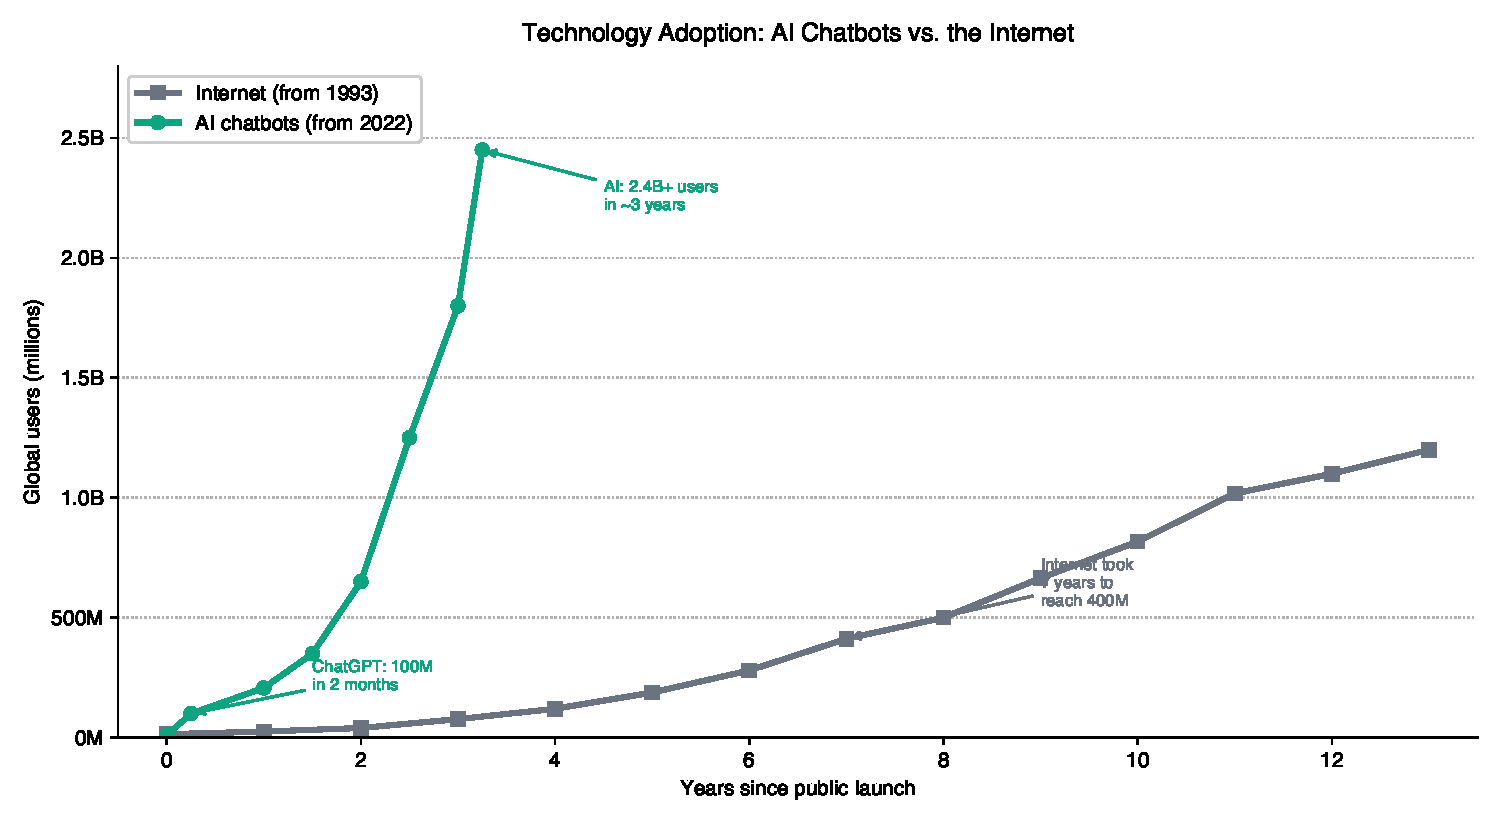
\includegraphics[width=\linewidth]{ai_platform_adoption}\\[0.3em]
{\scriptsize ChatGPT reached 100M users in two months --- the fastest consumer technology
adoption in history. Source: Feng, Miao \& Yuan (forthcoming).}
\end{center}
\end{column}
\begin{column}{0.48\textwidth}
\begin{center}
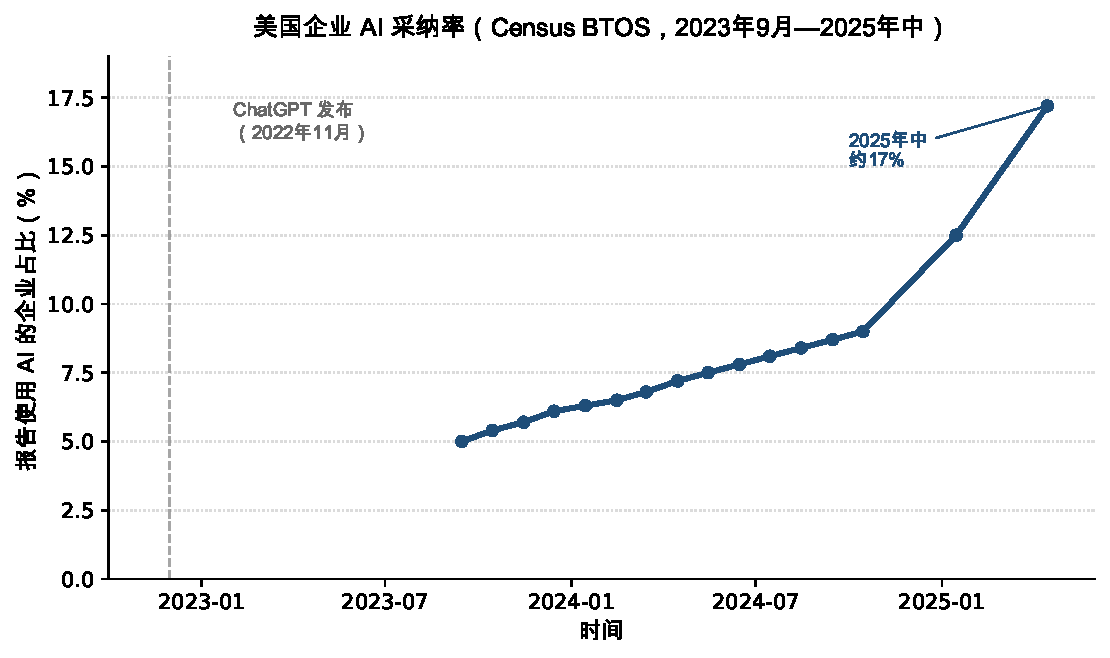
\includegraphics[width=\linewidth]{ch10_btos_ai_adoption}\\[0.3em]
{\scriptsize U.S.\ business AI adoption (Census Bureau BTOS), 2023--2024: rapid diffusion
across sectors and firm sizes. Source: Feng, Miao \& Yuan (forthcoming).}
\end{center}
\end{column}
\end{columns}
\end{frame}

\begin{frame}{AI Capability and Cost: Two Compounding Tailwinds}
\begin{columns}[T]
\begin{column}{0.48\textwidth}
\begin{center}
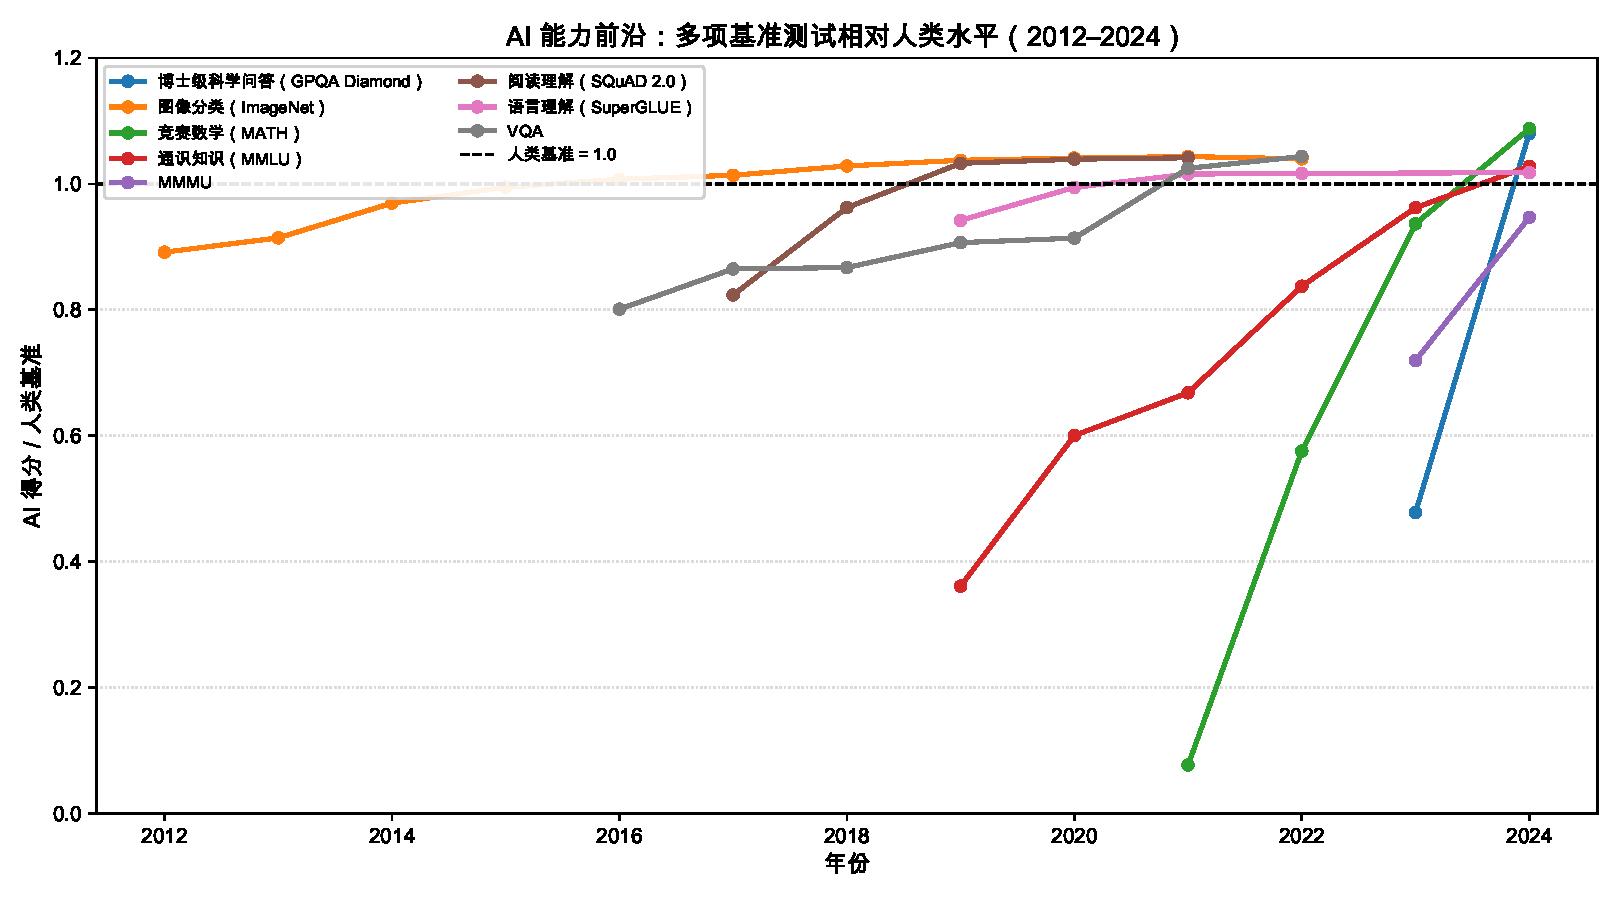
\includegraphics[width=\linewidth]{ch10_ai_performance}\\[0.3em]
{\scriptsize AI benchmark performance, 2012--2024: AI now \emph{exceeds} human baselines on
most standard tasks. Source: Stanford AI Index; Feng, Miao \& Yuan (forthcoming).}
\end{center}
\end{column}
\begin{column}{0.48\textwidth}
\begin{center}
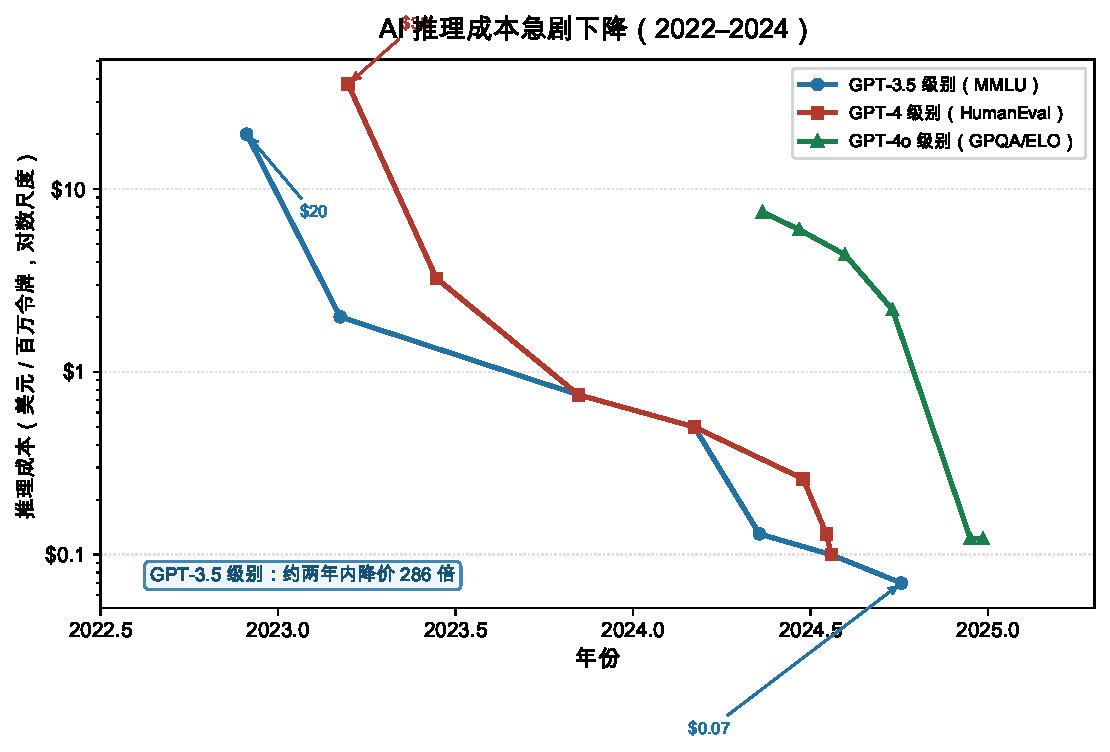
\includegraphics[width=\linewidth]{ai_cost_performance}\\[0.3em]
{\scriptsize Inference cost has fallen $\sim$280$\times$ in three years; capabilities have
compounded simultaneously. Source: Feng, Miao \& Yuan (forthcoming).}
\end{center}
\end{column}
\end{columns}
\vspace{0.4em}
\begin{block}{}
\small Rising capability $\times$ falling cost $=$ explosive economic penetration.
\end{block}
\end{frame}

\begin{frame}{AI's Footprint in the Labor Market: Distributional Exposure}
\begin{columns}[T]
\begin{column}{0.48\textwidth}
\begin{center}
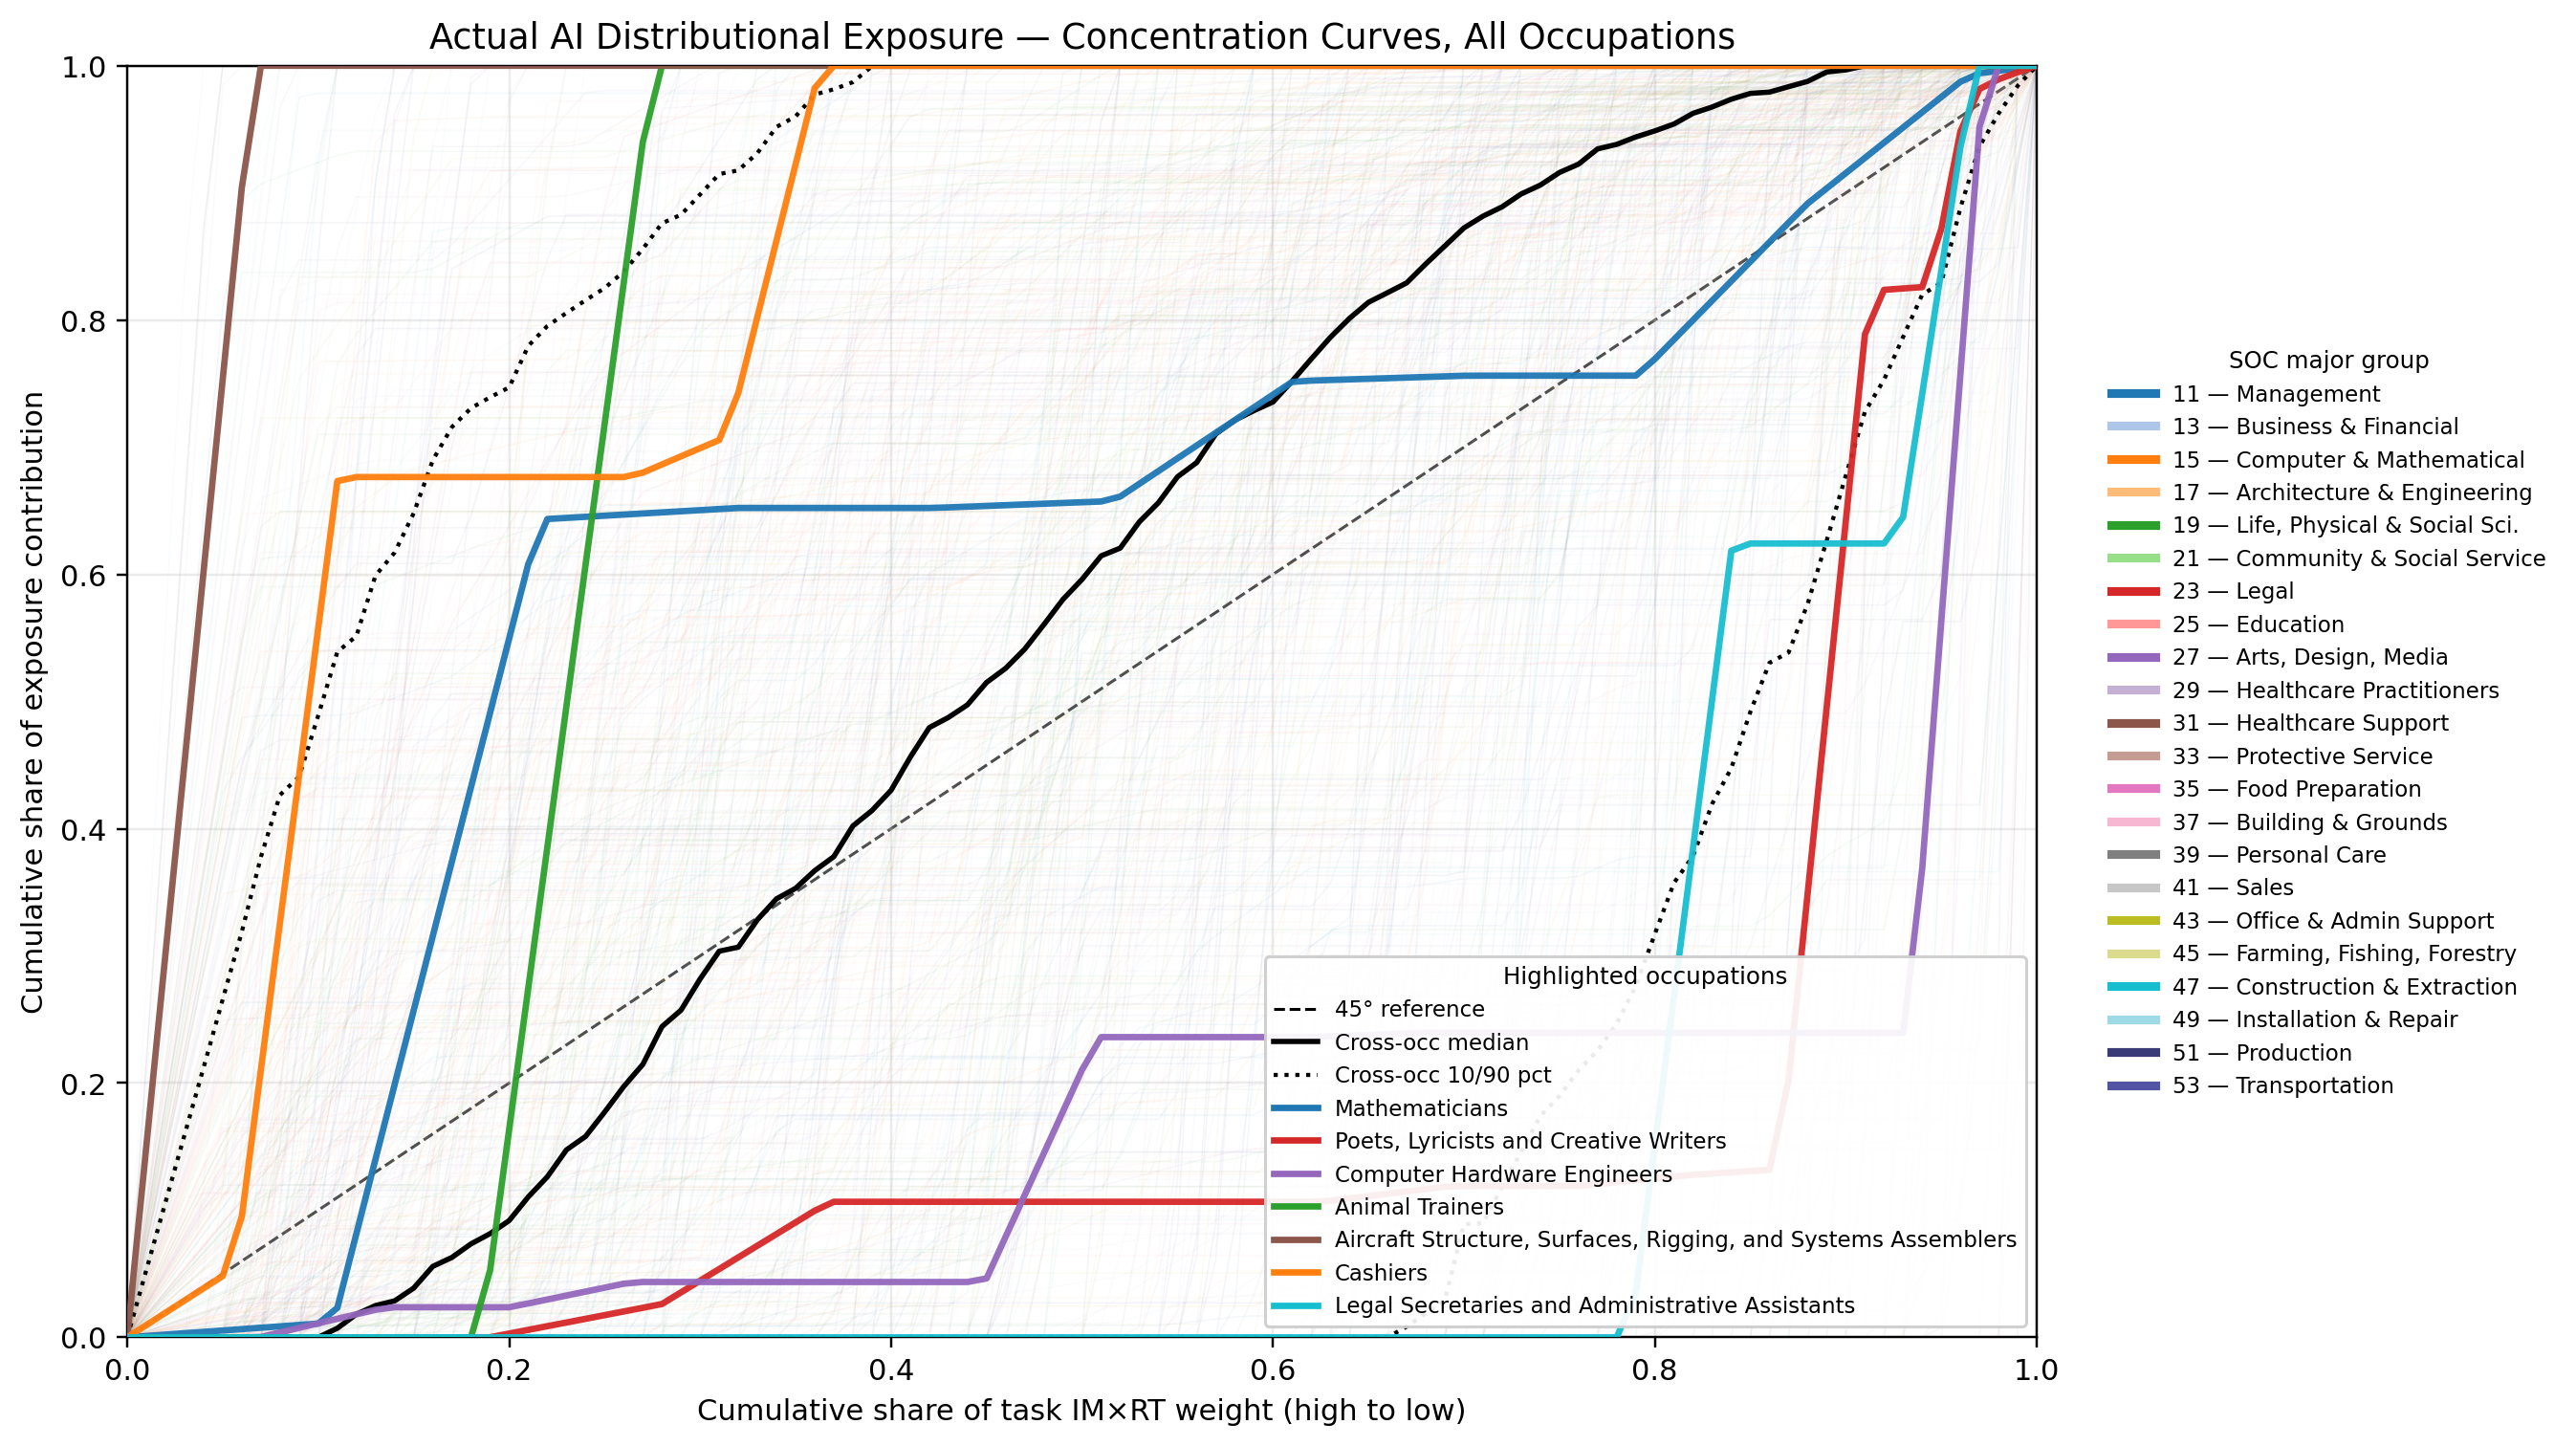
\includegraphics[width=\linewidth]{spaghetti_distributional_exposure_actual}\\[0.2em]
{\scriptsize \textbf{Actual AI concentration curves, 833 occupations.}
Each curve: cumulative AI usage share vs.\ cumulative task importance weight (tasks ranked
by O*NET importance, high to low). Above the 45$^\circ$ line: AI on \emph{core} tasks.
Below: AI on \emph{peripheral} tasks. Source: Feng et al.\ (2026).}
\end{center}
\end{column}
\begin{column}{0.49\textwidth}
\small
\textbf{How the measure is built:}
\begin{itemize}\setlength\itemsep{0.5em}
  \item \textbf{Tasks:} O*NET occupational task lists with importance weights (1--5 scale)
  \item \textbf{AI exposure:} actual Claude API usage share per task type
  \item \textbf{Concentration:} for each occupation, plot the Lorenz-style curve;
        the \textbf{Gini $G$} summarizes whether AI concentrates on core or peripheral tasks
\end{itemize}
\medskip
\textbf{What it says:}
\begin{itemize}\setlength\itemsep{0.5em}
  \item $G > 0$: AI on \textbf{core tasks} --- deep workplace integration
  \item $G < 0$: AI on \textbf{peripheral tasks} --- surface engagement
  \item Wide dispersion across 833 occupations: AI penetration is highly
        \textbf{heterogeneous} across the labor market
\end{itemize}
\end{column}
\end{columns}
\end{frame}

% ============================================================
\section{Overview}
% ============================================================

\begin{frame}{Overview}
\textbf{Research question.} Under incomplete markets and idiosyncratic employment risk,
what does \textbf{Ramsey optimal taxation} imply for \textbf{public debt}, the
\textbf{government's role as House of Finance}, and \textbf{long-run fiscal dynamics}?

\medskip
We pursue this by extending a representative-agent deep Ramsey solver (debt sustainability,
endogenous admissible sets) to a heterogeneous-agent economy --- with AI compressing the
model--algorithm--code loop along the way.

\medskip
\begin{enumerate}
  \item \textbf{The workflow} --- homotopy from one research paper to the next
  \item \textbf{The seed} --- representative-agent Ramsey taxation and debt sustainability
  \item \textbf{Opening the conversation} --- how the AI collaboration was structured
  \item \textbf{Milestones} --- refined RA $\to$ stripped-down HA $\to$ full HA $\to$ new discoveries
  \item \textbf{The final product} --- the HA Ramsey model, algorithm, and codebase
  \item \textbf{Major findings} --- debt limits and ergodic dynamics (RA) vs.\ House of Finance and bistability (HA)
  \item \textbf{Lessons} --- what this paradigm shift demands from the researcher
\end{enumerate}
\end{frame}

\begin{frame}{Public Debt as House of Finance}
\textbf{The central reframing in the HA model:}

\medskip
In the \textbf{representative-agent} model, public debt has one role: \textbf{tax smoothing}
--- spread the cost of spending shocks over time (Barro 1979; Lucas--Stokey 1983).

\medskip
In the \textbf{heterogeneous-agent} model, debt plays a second, deeper role:

\medskip
\begin{block}{The House of Finance}
Government bonds are the \textbf{only liquid asset} households can use to self-insure against
idiosyncratic employment risk. The Ramsey planner must manage the \emph{supply} of this
financial instrument --- not only the tax path.
\end{block}

\medskip
\begin{itemize}
  \item \textbf{Transition:} the planner deliberately \emph{builds up} bond supply early,
        issuing debt at a labor-tax \emph{subsidy}; households accumulate reserves
  \item \textbf{Long run:} if bond supply is insufficient at the start,
        the economy drifts toward immiseration --- the house of finance is never built
  \item \textbf{Implication:} managing the \emph{level} of public debt is inseparable from
        enabling household self-insurance
\end{itemize}
\end{frame}

\begin{frame}{What This Paper Delivers}
\compacttables
\begin{center}\footnotesize
\begin{tabular}{p{3.4cm}p{4.2cm}p{4.8cm}}
\toprule
\textbf{Layer} & \textbf{Started with} & \textbf{Ended with} \\
\midrule
Economic model & RA Ramsey taxation, incomplete markets (Feng--Han--Zhu) & HA Ramsey with employment risk and borrowing constraints (Chien--Feng--Wen) \\
Algorithm & Two-level fixed point; admissible set as DNN classifier & Viability kernel via $\alpha$-shapes; FB complementarity; Lyapunov-type penalty \\
Code & Working PyTorch RA solver & Full HA research codebase (\texttt{v1} $\to$ \texttt{v2\_fullmodel}) \\
\bottomrule
\end{tabular}
\end{center}

\smallskip
\begin{block}{}
All three layers --- model, algorithm, code --- were grown \emph{together}, with AI compressing
the loop between them. The audit trail lives in \texttt{Case\_Study/}.
\end{block}
\end{frame}

% ============================================================
\section{The Workflow}
% ============================================================

\begin{frame}{The Homotopy Workflow}
\textbf{Solve an easier version first, validate it, then continuously grow it toward the full research task.}

\medskip
\begin{center}
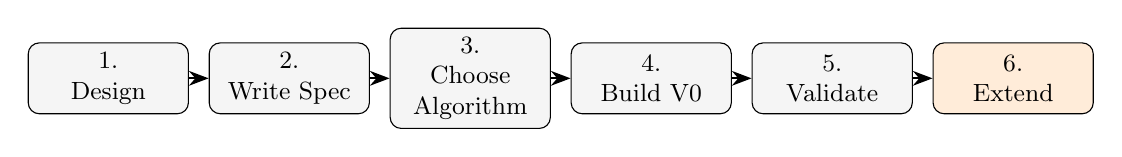
\begin{tikzpicture}[
    box/.style={rectangle, draw=black, fill=VeryLightGray, rounded corners,
                minimum width=1.9cm, minimum height=0.9cm,
                text width=1.8cm, align=center, font=\small},
    arrow/.style={-{Stealth[length=2.5mm]}, thick}
]
    \node[box] (design) {1.\\Design};
    \node[box, right=0.25cm of design] (spec) {2.\\Write Spec};
    \node[box, right=0.25cm of spec] (algo) {3.\\Choose Algorithm};
    \node[box, right=0.25cm of algo] (v0) {4.\\Build V0};
    \node[box, right=0.25cm of v0] (val) {5.\\Validate};
    \node[box, right=0.25cm of val, fill=orange!15] (ext) {6.\\Extend};
    \draw[arrow] (design) -- (spec);
    \draw[arrow] (spec) -- (algo);
    \draw[arrow] (algo) -- (v0);
    \draw[arrow] (v0) -- (val);
    \draw[arrow] (val) -- (ext);
\end{tikzpicture}
\end{center}

\medskip
\begin{itemize}
    \item Start from a version with clear intuition and known checks
    \item Add one new margin at a time; attribute new bugs to the new margin
    \item Never ask the agent to ``solve the full complicated problem'' in one jump
\end{itemize}

\medskip
\textbf{This paper's instance:} the ``V0'' is not a toy --- it is a complete, published-quality RA solver.
The homotopy runs from one research paper to the next.
\end{frame}

\begin{frame}{Three Layers Grow Together}
\textbf{In computational research, all three layers must grow in step:}

\smallskip
\begin{center}
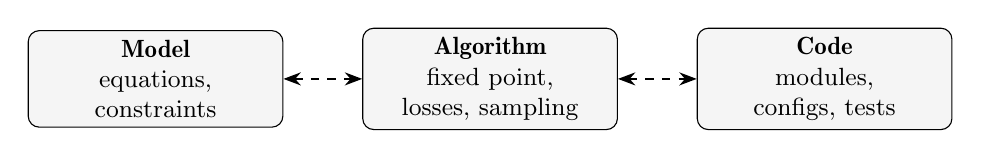
\begin{tikzpicture}[
    lay/.style={rectangle, draw=black, fill=VeryLightGray, rounded corners,
                minimum width=3.1cm, minimum height=0.8cm,
                text width=3.0cm, align=center, font=\small},
    da/.style={{Stealth[length=2.2mm]}-{Stealth[length=2.2mm]}, thick, dashed}
]
    \node[lay] (m) {\textbf{Model}\\ equations, constraints};
    \node[lay, right=1.0cm of m] (alg) {\textbf{Algorithm}\\ fixed point, losses, sampling};
    \node[lay, right=1.0cm of alg] (c) {\textbf{Code}\\ modules, configs, tests};
    \draw[da] (m) -- (alg);
    \draw[da] (alg) -- (c);
\end{tikzpicture}
\end{center}

\smallskip
\begin{itemize}\small\itemsep2pt
    \item A new model element (borrowing constraints) forces a new algorithmic element
          (complementarity penalties), which forces new code (FB residuals in the loss)
    \item Discoveries also flow \emph{backwards}: a numerical pathology (divergent rollouts)
          revealed a missing theoretical object (the viability kernel)
    \item AI's role: keep the three layers \emph{synchronized} --- TeX, pseudocode, and PyTorch
          must always describe the same economy
\end{itemize}

\smallskip
\begin{block}{The homotopy path of this paper}
\small RA model/algorithm/code $\rightarrow$ stripped-down HA $\rightarrow$ full HA $\rightarrow$
HA $+$ geometric viability $+$ Lyapunov selection.
\end{block}
\end{frame}

\begin{frame}{What Makes a Good Seed?}
\textbf{The single most important input to this workflow is the starting artifact.}

\medskip
\begin{itemize}
    \item \textbf{It works.} The RA solver trains, simulates, and reproduces the paper's
          quantitative results --- every later failure is attributable to a change
    \item \textbf{It is documented.} A TeX file states the model and the algorithm in the
          same notation the code uses
    \item \textbf{It is modular.} Sampling, scoring, training, and simulation live in
          separate modules with a config file --- the agent can modify one without breaking the rest
    \item \textbf{It points somewhere.} The RA model is the natural degenerate case of the
          HA model (shut down idiosyncratic risk and heterogeneity)
\end{itemize}

\medskip
\begin{block}{}
A good seed is to agentic research what a good instrument is to empirical work:
most of the credibility is purchased before the main analysis starts.
\end{block}
\end{frame}

% ============================================================
\section{The Seed: RA Deep Ramsey Solver}
% ============================================================

\begin{frame}{The RA Model in One Slide}
\textbf{Ramsey optimal taxation with non-contingent debt} (Feng--Han--Zhu, \emph{Ramsey Taxation, Public Debt Sustainability, and Asset Pricing in Incomplete Markets}).

\smallskip
Representative household, linear technology $Y=L$, flat labor tax $\tau$, one-period bond at price $q$, Markov spending shock $G(z)$. Recursive Ramsey state: $(z, B, \lambda)$ with co-state $\lambda = u'(c)$.

\vspace{-0.1cm}
\[
V(z,B,\lambda) \;=\; \max_{\{\lambda_+(z_+)\}} \Big\{\, u(c) - h(l) + \beta\,\mathbb{E}\big[V(z_+, B_+, \lambda_+)\big] \Big\}
\]
subject to
\[
G(z)+B \le \tau l + q B_+, \qquad c + G(z) = l, \qquad (1-\tau)u'(c)=h'(l), \qquad q\,u'(c)=\beta\,\mathbb{E}[\lambda_+ \mid z],
\]
\[
\text{and the \emph{sustainability} requirement } (B,\lambda) \in \Omega(z).
\]

\smallskip
\begin{itemize}
    \item $\Omega(z)$: the set of debt/co-state pairs from which the government can stay solvent
          forever --- \textbf{endogenous and unknown a priori}
    \item \textbf{Quasi-linear case} $u(c)=c$: $\lambda \equiv 1$, $q=\beta$, state collapses to $(z,B)$;
          the marginal value of debt $V_B$ is a \emph{supermartingale}
\end{itemize}
\end{frame}

\begin{frame}[label=mainRAalgo]{The RA Algorithm: Two-Level Fixed Point}
\textbf{Three neural networks trained jointly} (PyTorch, actor--critic style):

\smallskip
\compacttables
\begin{center}\footnotesize
\begin{tabular}{p{1.5cm}p{4.4cm}p{5.8cm}}
\toprule
\textbf{Network} & \textbf{Object} & \textbf{Training signal} \\
\midrule
$f_\Lambda$ & policy: contingent co-states $\lambda_+(z_+)$ & maximize simulated welfare $+$ terminal value, penalty $\kappa\,[1-f_\Omega(S)]$ off the admissible set \\
$f_V$ & value function & MSE against realized discounted utility on rollouts \\
$f_\Omega$ & admissible set $\Omega$ & \textbf{binary classification}: label a state $1$ if its successor stays in $\Omega^{(n)}$ with finite value \\
\bottomrule
\end{tabular}
\end{center}

\smallskip
{\small\textbf{Outer iteration $n$:}}
\begin{enumerate}\small\itemsep1pt
    \item Given $\Omega^{(n)}$: update policy and value (rejection-sample states from $f_\Omega$, simulate, fit)
    \item Given the new policy: relabel sampled states, retrain $f_\Omega^{(n+1)}$
\end{enumerate}
\begin{block}{Key idea to carry forward}
\small Domain-finding is itself a fixed-point problem, solved \emph{jointly} with the policy.
\end{block}
\vspace{0.3em}\hfill
\hyperlink{appRAprob}{\beamergotobutton{Recursive Problem}}\hspace{0.4em}%
\hyperlink{appRAalgo}{\beamergotobutton{Algorithm Details}}
\end{frame}

\begin{frame}{The RA Codebase}
\textbf{Five modules plus one config --- the structure the agent will inherit:}

\smallskip
\compacttables
\begin{center}\footnotesize
\begin{tabular}{p{3.6cm}p{8.3cm}}
\toprule
\textbf{File} & \textbf{Role} \\
\midrule
\texttt{config.json} & all economics and hyperparameters: shocks, bounds, penalties, sampling, admissibility thresholds, simulation options \\
\texttt{dashboard.py} & orchestration: load config, create networks, sample, train \\
\texttt{adaptive\_sampling.py} & admissibility scoring, adaptive sampling, dynamic boundary updates \\
\texttt{value\_module.py} & policy/value networks, trainer, plotting utilities \\
\texttt{simulation.py} & post-training rollouts and figures \\
\texttt{pretrain.py} & optional pretraining from legacy solution data \\
\bottomrule
\end{tabular}
\end{center}

\smallskip
\begin{itemize}\small
    \item Configuration-driven design: every later experiment is a config diff, not a code fork
    \item In the RA case the feasible region is low-dimensional --- representable by debt bounds
          $B_{\min}(\mu,g)$, $B_{\max}(\mu,g)$ estimated within bins
    \item \textbf{This cheap representation is exactly what will break under heterogeneity}
\end{itemize}
\end{frame}

\begin{frame}{Why This Seed Could Grow}
\begin{columns}[T]
\begin{column}{0.55\textwidth}
\textbf{Extension potential, layer by layer:}
\begin{itemize}
    \item \emph{Model:} the RA economy is the no-risk limit of an economy with employed/unemployed
          households --- the HA model nests it
    \item \emph{Algorithm:} the two-level fixed point (policy $\leftrightarrow$ domain) carries over
          unchanged in spirit; only the \emph{representation} of $\Omega$ must change
    \item \emph{Code:} actor--critic loop, config plumbing, simulation and plotting all reusable
\end{itemize}
\end{column}
\begin{column}{0.42\textwidth}
\textbf{What is genuinely missing:}
\begin{itemize}
    \item High-dimensional state (5D vs.\ 2--3D)
    \item Occasionally binding borrowing constraints (complementarity, not box penalties)
    \item A geometric representation of the admissible set
    \item Equilibrium-selection machinery for unit-root dynamics
\end{itemize}
\end{column}
\end{columns}

\medskip
\begin{block}{}
The gap list above \emph{is} the research plan. Each missing item became a milestone
in the AI collaboration --- and two of them became new discoveries.
\end{block}
\end{frame}

% ============================================================
\section{Opening the Conversation}
% ============================================================

\begin{frame}{The Package Is the Context}
\textbf{The collaboration record lives in \texttt{Case\_Study/} --- organized so any researcher can reconstruct every step:}

\smallskip
\compacttables
\begin{center}\footnotesize
\begin{tabular}{p{5.9cm}p{6.0cm}}
\toprule
\textbf{Folder / file} & \textbf{Role} \\
\midrule
\texttt{.../RA\_Ramsey\_NN\_original/} & the seed: working RA solver \\
\texttt{.../RA\_local\_refined\_v2/} & Milestone 1: refined RA code \\
\texttt{.../HA\_Ramsey\_HA\_NN/v1/} & Milestone 3: first HA prototype \\
\texttt{.../HA\_Ramsey\_HA\_NN/v2\_fullmodel/} & Milestone 4: full HA implementation \\
\texttt{02\_tex\_model\_algorithm\_growth/} & TeX tracking model/algorithm versions \\
\texttt{03\_notes\_and\_audits/} & code-vs-document audits, dialogue notes \\
\texttt{deep\_ramsey\_ai\_case\_study.md} & the narrative this talk is based on \\
\bottomrule
\end{tabular}
\end{center}

\smallskip
\begin{itemize}\small
    \item Theory TeX and code are kept \emph{side by side} so every equation can be checked in both places
    \item Conversation provenance (chat links) is recorded, but local files are the citable artifacts
\end{itemize}
\end{frame}

\begin{frame}[fragile]{The First Prompts: Restate, Then Audit}
\textbf{The conversation did not start with ``build me an HA model.'' It started with comprehension and audit tasks on the seed:}

\begin{lstlisting}[basicstyle=\ttfamily\scriptsize,numbers=none]
1. "Here are the RA paper (TeX) and the RA repository.
    Restate the model and the algorithm in your own words.
    List every equation and where it is implemented."

2. "Audit the code against the document. Report every place
    where the code and the TeX disagree: scoring, bounds,
    sampling, penalties. Classify each as a correctness risk
    or a documentation gap."

3. "Propose a refined RA document + code pair in which the
    two are consistent. Do not add any new economics yet."
\end{lstlisting}

\smallskip
\begin{itemize}\small
    \item Output of step 2 is preserved: \texttt{03\_notes\_and\_audits/code\_vs\_document\_analysis.md}
\end{itemize}
\begin{block}{Why audit first?}
\small Extending an inconsistent seed propagates the inconsistency
into every later version. The audit is the cheapest insurance in the whole project.
\end{block}
\end{frame}

\begin{frame}{The Division-of-Labor Contract}
\textbf{Set expectations explicitly at the start --- who owns what:}

\smallskip
\compacttables
\begin{center}\footnotesize
\renewcommand{\arraystretch}{1.0}
\begin{tabular}{p{6.6cm}cc}
\toprule
\textbf{Contribution} & \textbf{AI} & \textbf{Economist} \\
\midrule
Drafting and reorganizing LaTeX formulations & \checkmark & \\
Translating equations into vectorized PyTorch & \checkmark & \\
Proposing FB-penalty and boundary-learning patterns & \checkmark & \\
Summarizing diagnostics and code/document mismatches & \checkmark & \\
Checking economic correctness of formulations & & \checkmark \\
Deciding which simplifications are acceptable & & \checkmark \\
Catching conceptual bugs (timing, transition direction) & & \checkmark \\
Setting validation benchmarks; accepting results & & \checkmark \\
\bottomrule
\end{tabular}
\end{center}

\smallskip
\begin{block}{}
\small The AI supplies \textbf{throughput}; the economist supplies \textbf{judgment} ---
the central lesson of the case study, stated before any code was written.
\end{block}
\end{frame}

% ============================================================
\section{Milestones}
% ============================================================

\begin{frame}{The Milestone Ladder}
\begin{center}
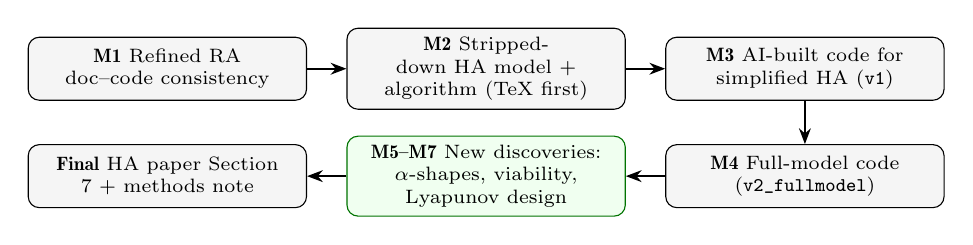
\begin{tikzpicture}[
    ms/.style={rectangle, draw=black, fill=VeryLightGray, rounded corners,
              minimum height=0.8cm, text width=3.3cm, align=center, font=\scriptsize},
    nd/.style={rectangle, draw=green!45!black, fill=green!6, rounded corners,
              minimum height=0.8cm, text width=3.3cm, align=center, font=\scriptsize},
    a/.style={-{Stealth[length=2mm]}, thick}
]
    \node[ms] (m1) {\textbf{M1} Refined RA\\ doc--code consistency};
    \node[ms, right=0.5cm of m1] (m2) {\textbf{M2} Stripped-down HA model + algorithm (TeX first)};
    \node[ms, right=0.5cm of m2] (m3) {\textbf{M3} AI-built code for simplified HA (\texttt{v1})};
    \node[ms, below=0.55cm of m3] (m4) {\textbf{M4} Full-model code (\texttt{v2\_fullmodel})};
    \node[nd, left=0.5cm of m4] (m5) {\textbf{M5--M7} New discoveries:\\ $\alpha$-shapes, viability, Lyapunov design};
    \node[ms, left=0.5cm of m5] (m8) {\textbf{Final} HA paper Section 7 + methods note};
    \draw[a] (m1) -- (m2);
    \draw[a] (m2) -- (m3);
    \draw[a] (m3) -- (m4);
    \draw[a] (m4) -- (m5);
    \draw[a] (m5) -- (m8);
\end{tikzpicture}
\end{center}

\medskip
\begin{itemize}
    \item Each milestone is a \emph{validated} artifact preserved in \texttt{Case\_Study/} ---
          the homotopy discipline applied at research scale
    \item Green box: where iteration with AI surfaced objects that became
          \textbf{contributions in their own right}
\end{itemize}
\end{frame}

\begin{frame}{M1: Refine the Seed Before Extending It}
\textbf{First deliverable: a revised RA algorithm and code, with the document and the implementation in exact agreement.}

\medskip
\begin{itemize}
    \item Artifacts: \texttt{RA\_model\_refine\_3.tex}, \texttt{deep\_ramsey\_refined\_v3.tex},
          and the aligned code copy \texttt{RA\_local\_refined\_v2/}
    \item The audit had found: scoring mismatches, boundary-learning details that differed
          between TeX and code, and scaling issues
    \item AI rewrote both sides; the economist adjudicated which side was \emph{right}
          when they disagreed
\end{itemize}

\medskip
\begin{exampleblock}{Typical fix}
The document described admissibility with a smooth power-barrier score;
the code used a different functional form. The refined pair uses the same barrier in both ---
so later HA scores could be derived from a trusted template.
\end{exampleblock}

\medskip
\textbf{Workflow point:} this milestone added \emph{zero} new economics. Resist the urge to skip it.
\end{frame}

\begin{frame}[label=mainM2]{M2: The New Model, Stripped Down (TeX Before Code)}
\textbf{Add heterogeneity: employed ($e$) / unemployed ($u$) households, idiosyncratic employment risk, incomplete markets, borrowing constraints.}

\smallskip
Five-dimensional state and three controls:
\[
s = (K,\, a^e,\, a^u,\, c^e,\, c^u), \qquad \text{actor outputs } (n^e,\, c'^e,\, c'^u)
\]
Everything else is derived in one explicit forward pass (separable CRRA, Cobb--Douglas):
\[
K' = K^{\alpha}(\pi^e n^e)^{1-\alpha} + (1-\delta)K - \pi^e c^e - \pi^u c^u, \qquad
Q = \beta\, (c^e)^{\sigma}\big[(c'^e)^{-\sigma}\pi^{ee} + (c'^u)^{-\sigma}\pi^{ue}\big]
\]
\[
a'^e = \tfrac{1}{Q}\Big[\tfrac{a^e \pi^e \pi^{ee} + a^u \pi^u \pi^{eu}}{\pi^e} + \hat{w}\, n^e - c^e\Big],
\qquad
a'^u = \tfrac{1}{Q}\Big[\tfrac{a^e \pi^e \pi^{ue} + a^u \pi^u \pi^{uu}}{\pi^u} - c^u\Big]
\]

\smallskip
\begin{alertblock}{Two conceptual bugs the economist caught}
AI-drafted, syntactically plausible equations:
(1) asset transitions must use \emph{current} consumption $c^e, c^u$ --- the budget constraint is a
current-period restriction; (2) transition probabilities must follow the \emph{direction of movement}
between employment states ($\pi^{ee}$ vs.\ $\pi^{ue}$ etc.). No compiler catches these.
\end{alertblock}
\vspace{0.2em}\hfill\hyperlink{appHAmodel}{\beamergotobutton{Model Details}}
\end{frame}

\begin{frame}[label=mainM2fb]{M2 (cont.): Borrowing Constraints as Complementarity}
\textbf{The genuinely new algorithmic ingredient: occasionally binding constraints.}

\smallskip
For each type $i \in \{e,u\}$, with Euler discrepancy $\phi^i$:
\[
a'^i \ge 0, \qquad \phi^i \ge 0, \qquad \phi^i \, a'^i = 0
\]
Embedded in a differentiable loss via the smoothed \textbf{Fischer--Burmeister} function:
\[
\Phi_\varepsilon(a,b) = a + b - \sqrt{a^2 + b^2 + \varepsilon^2}, \qquad
\text{actor loss} = -\,\mathbb{E}[\text{value}] + \lambda_{FB}\,\mathbb{E}\big[\Phi_\varepsilon(\phi^e, a'^e)^2 + \Phi_\varepsilon(\phi^u, a'^u)^2\big]
\]

\smallskip
\begin{itemize}
    \item $\lambda_{FB}$ follows an augmented schedule: start moderate (let the policy explore),
          multiply by $\rho$ whenever average FB residuals stay above tolerance
    \item The FB residual becomes a \emph{first-class diagnostic}: it measures directly whether
          complementarity is actually satisfied
    \item Strategic simplification: log utility, symmetric transitions, simple calibration ---
          \textbf{simplicity is a design decision, not a limitation}
\end{itemize}
\vspace{0.2em}\hfill\hyperlink{appHArec}{\beamergotobutton{Recursive Problem + KKT}}
\end{frame}

\begin{frame}{M3: AI Builds the Code for the Simplified HA Model (\texttt{v1})}
\textbf{With the TeX spec fixed, the agent produced the first running HA prototype.}

\smallskip
\compacttables
\begin{center}\footnotesize
\begin{tabular}{p{3.0cm}p{8.9cm}}
\toprule
\textbf{Module} & \textbf{Contents} \\
\midrule
\texttt{ha\_model.py} & actor/critic networks; 5D forward pass; FB residuals; admissibility score \\
\texttt{boundary.py} & first $\alpha$-boundary learner (Delaunay $+$ circumradius filter) \\
\texttt{dashboard.py} & compact loop ($\approx$250 lines): boundary update $\to$ critic $\to$ actor $\to$ FB schedule \\
\texttt{simulation.py} / \texttt{visualization.py} & Monte Carlo rollouts, basic plots \\
\texttt{config.json} & all parameters, bounds, schedules \\
\bottomrule
\end{tabular}
\end{center}

\smallskip
\begin{itemize}\small
    \item Same module skeleton as the RA seed --- deliberate, so diffs stay interpretable
    \item Validation gate: forward pass reproduces hand-derived transitions; FB residuals
          shrink under the penalty schedule; admissible region looks economically sensible
\end{itemize}

\smallskip
\textbf{Status at M3: a proof of concept, not yet a research instrument.}
\end{frame}

\begin{frame}{M4: The Full Model (\texttt{v2\_fullmodel}) --- Debugging Becomes Architecture}
\textbf{Each numerical failure of \texttt{v1} was encoded as explicit structure in \texttt{v2}} (\texttt{dashboard.py} grows from $\approx$250 to $>$1{,}200 lines):

\smallskip
\compacttables
\begin{center}\footnotesize
\renewcommand{\arraystretch}{1.0}
\begin{tabular}{p{5.5cm}p{6.4cm}}
\toprule
\textbf{Failure discovered in \texttt{v1}} & \textbf{\texttt{v2\_fullmodel} response} \\
\midrule
Naive 5D sampling: low admissibility pass rates & adaptive loops keep sampling until enough valid points accumulate \\
Fragile boundary estimates in 5D & normalized coordinates, Delaunay \texttt{QJ} joggling, save/reload of the $\alpha$-shape \\
Rollouts escape the learned admissible set & \texttt{project\_to\_admissible} ($\Pi_\Omega$) $+$ projection-distance penalty \\
Critic bootstrapping instability & frozen target critic with soft updates \\
``Something is wrong'' is not actionable & separate tracking of value, FB, boundary, shape, total losses \\
Period 0 differs from continuation & explicit period-0 allocation problem in simulation \\
\bottomrule
\end{tabular}
\end{center}
\begin{block}{}
\small The explicit \textbf{Level-1 (stabilize domain) / Level-2 (optimize policy)} loop emerged here ---
the code finally matched the two-level fixed-point theory of the RA document.
\end{block}
\end{frame}

\begin{frame}{M5 --- New Discovery I: $\alpha$-Shapes for the Feasible Set}
\textbf{Problem:} in 5D, debt-bound functions and grids are hopeless. The admissible set must be represented \emph{geometrically} from sampled points.

\medskip
\textbf{Solution} (Edelsbrunner--M\"ucke 1994): the \emph{$\alpha$-shape} of the admissible point cloud ---
the union of Delaunay simplices with circumradius $\le 1/\alpha$.

\medskip
\begin{columns}[T]
\begin{column}{0.55\textwidth}
\begin{itemize}
    \item $\alpha \to 0$: convex hull; \; $\alpha \to \infty$: the bare point set ---
          $\alpha$ tunes how much non-convexity is admitted
    \item Crucial because the HA feasible set is \textbf{generically non-convex}
          (the borrowing-constraint kink)
    \item Pipeline: normalize $\to$ Delaunay $\to$ circumradius filter $\to$
          \texttt{find\_simplex} membership $\to$ KD-tree buffer
\end{itemize}
\end{column}
\begin{column}{0.42\textwidth}
\begin{exampleblock}{How it surfaced}
The agent's first boundary learner kept misclassifying
near-kink states. Iterating on \emph{why} led from ad hoc fixes to the computational-geometry
literature --- a tool import economists rarely make.
\end{exampleblock}
\end{column}
\end{columns}

\medskip
\textbf{Where it lives:} \texttt{boundary.py} (\texttt{AlphaBoundary}); written up in the methods
note \texttt{computational\_Ramsey.tex} and the HA paper, Section 7.
\end{frame}

\begin{frame}{M6 --- New Discovery II: Viability Precedes Admissibility}
\textbf{What \emph{is} the set the $\alpha$-shape approximates? Iterating with AI on this question connected two literatures.}

\smallskip
{\small The admissible set is a \textbf{viability kernel} in the sense of Aubin (1991) --- the
\emph{largest} set of states from which a feasible trajectory exists indefinitely:}
\vspace{-0.1cm}
\[
\small
\Omega = \big\{ s \in H : \exists\, y \ \text{s.t.}\ s' = f(s,y) \in \Omega \ \text{and feasibility/KKT hold} \big\},
\]
\vspace{-0.55cm}
\[
\small
\mathcal{T}(D) = \big\{ s \in D : \exists\, y \ \text{s.t.}\ f(s,y) \in D,\ \text{constraints hold} \big\},
\qquad D^0 = H,\quad D^{k+1} = \mathcal{T}(D^k) \downarrow \Omega^{*}.
\]

\smallskip
\begin{block}{The connection}
\small The same abstract structure as \emph{self-generation} in
APS (Abreu--Pearce--Stacchetti, \emph{Econometrica} 1990) --- equilibrium sets as the largest
fixed point of a monotone set operator, computed by downward iteration; used for Ramsey problems
by Phelan--Stacchetti (2001) and Feng (2015). \textbf{The math literature on viability
precedes the economics literature on admissibility.}
\end{block}

\smallskip
{\small Practical payoff: grid-based set iteration (Saint-Pierre 1994; Feng 2015) is replaced by
$\alpha$-shapes over \emph{unstructured point clouds} --- sidestepping the curse of dimensionality.}
\end{frame}

\begin{frame}{M7 --- New Discovery III: A Lyapunov-Type Penalty for Saddle-Path Selection}
{\small\textbf{Problem:} with $\beta R = 1$ in the long run, the HA Ramsey dynamics have a \emph{unit root}:
a continuum of quasi-steady states along the full-insurance ridge. Rollouts drift or explode;
the optimizer cannot tell the saddle path from divergence.}

\smallskip
{\small\textbf{Solution: a level-independent Lyapunov-type penalty} --- flat along the unit-root
direction, punishing only movement that signals instability:}
\vspace{-0.1cm}
\[
\small
\mathcal{P}_{\text{lyap}} \;=\; \sum_t \beta^t \Big[\, w_{\text{spread}}\,\big(c^e_t - c^u_t\big)^2
\;+\; \big[\,a^{tot}_t - a^{tot}_{t-1}\,\big]_+^2 \,\Big]
\]
\vspace{-0.35cm}
\begin{itemize}\small
    \item First term: penalize the \emph{consumption spread}, zero on the $c^e = c^u$ ridge ---
          selects convergence to full insurance without pinning the level
    \item Second term: penalize \emph{explosive asset growth} (one-sided), leaving the unit-root level free
    \item Not a formal certificate --- a \emph{training-objective} use of Lyapunov logic;
          to our knowledge new in Ramsey computation
\end{itemize}

\smallskip
\begin{exampleblock}{How it surfaced}
\small Repeated failed training runs $\to$ AI-generated diagnostics isolating the
unstable directions $\to$ the economist recognized a saddle-path problem $\to$ joint design
of a penalty with the right invariance properties.
\end{exampleblock}
\end{frame}

% ============================================================
\section{The Final Product}
% ============================================================

\begin{frame}{Final Model: HA Ramsey with Employment Risk}
\textbf{Chien--Feng--Wen, \emph{Understanding Optimal Ramsey Policies in Heterogeneous-Agents Economies}, Section 7.}

\medskip
\begin{columns}[T]
\begin{column}{0.52\textwidth}
\textbf{Environment (quantitative section):}
\begin{itemize}
    \item Employed/unemployed households; ex-ante identical, ex-post heterogeneous
    \item Symmetric i.i.d.\ employment risk ($\pi(e|u)=\pi(u|e)=\tfrac12$)
    \item Borrowing constraint on the unemployed; government bonds the only asset
    \item Linear technology ($\alpha=\delta=0$): effective state is 4D, $s=(a^e, a^u, c^e, c^u)$
\end{itemize}
\end{column}
\begin{column}{0.45\textwidth}
\textbf{Preferences:}
\[
u(c,n) = \frac{c^{1-\sigma}}{1-\sigma} - \frac{n^{1+\gamma}}{1+\gamma}
\]
CRRA benchmark $\sigma=\gamma=2$, $\beta=0.8$; GHH variant for comparison.

\medskip
\textbf{Promised consumptions} $(c^e, c^u)$ carried as states: the recursive device for
Ramsey commitment, inherited from the RA formulation.
\end{column}
\end{columns}

\smallskip
\begin{itemize}\small
    \item Ramsey planner chooses labor tax and debt under full commitment, internalizing
          households' self-insurance behavior
    \item \textbf{New role for public debt}: not only tax smoothing (RA), but the supply of
          \emph{liquid assets} for self-insurance
\end{itemize}
\end{frame}

\begin{frame}[label=mainFinalAlgo]{Final Algorithm: The Enforcement Stack}
\textbf{Nested fixed point over (actor $\theta$, critic $\psi$, domain $\Omega$)} --- the matured version of the RA two-level idea:

\smallskip
\compacttables
\begin{center}\footnotesize
\renewcommand{\arraystretch}{1.0}
\begin{tabular}{p{2.0cm}p{9.9cm}}
\toprule
\textbf{Level 1} & sample from hypercube $H$; score admissibility
$\mathcal{A}(s;\theta,\Omega) = w_{geo}\mathbf{1}\{f_\theta(s)\in\Omega\} + w_Q\,\mathcal{B}(Q^{raw})$;
rebuild $\Omega$ as the $\alpha$-shape of high-scoring states \\
\textbf{Level 2} & form the admissible training pool; critic: TD error on rollouts;
actor: welfare $-$ FB complementarity $-$ Euler-sign $-$ projection-distance
$-$ Lyapunov-type penalties \\
\bottomrule
\end{tabular}
\end{center}

\smallskip
\begin{itemize}\small
    \item Rollouts are projected back: $s_{t+1} = \Pi_\Omega\big(f_\theta(s_t)\big)$, with the
          projection distance penalized
    \item Amortized updates (domain refreshed every $\sim$20 iterations) tame the
          non-stationarity of learning on a moving domain
    \item Hyperparameters disciplined by systematic sweeps (32$+$ configurations) ---
          AI agents ran and summarized the sweeps
\end{itemize}

\smallskip
\begin{block}{}
\small Every component answers a specific failure met along the way. The algorithm \emph{is}
the accumulated debugging history, made explicit.
\end{block}
\vspace{0.2em}\hfill
\hyperlink{appFB}{\beamergotobutton{Complementarity}}\hspace{0.3em}%
\hyperlink{appDomain}{\beamergotobutton{Domain Learning}}\hspace{0.3em}%
\hyperlink{appLyap}{\beamergotobutton{Lyapunov}}\hspace{0.3em}%
\hyperlink{appStack}{\beamergotobutton{Full Stack}}
\end{frame}

\begin{frame}{Final Codebase and Provenance}
\compacttables
\begin{center}\footnotesize
\begin{tabular}{p{4.2cm}p{7.7cm}}
\toprule
\textbf{Artifact} & \textbf{Status} \\
\midrule
\texttt{v2\_fullmodel/} code & full HA research code path: versioning, checkpoints, target critic, Level-1/2 loop, period-0 simulation, rich diagnostics \\
\texttt{computational\_Ramsey.tex} & standalone methods note: viability, $\alpha$-shapes, FB stack, sweep evidence \\
HA paper, Section 7 & quantitative results: transitions, basins of attraction, CRRA vs.\ GHH \\
\texttt{Case\_Study/} package & the audit trail: every milestone's code, TeX, and notes \\
\bottomrule
\end{tabular}
\end{center}

\smallskip
{\small\textbf{The same triple we started with --- model, algorithm, code --- but now for a new economy, with genuinely new methodological components and a paper trail connecting every step.}}

\smallskip
\begin{block}{}
\small Time from seed to working full HA solver: weeks, not years. The binding constraint
was economist judgment at the milestones, not implementation labor.
\end{block}
\end{frame}

% ============================================================
\section{Major Findings}
% ============================================================

\begin{frame}{RA Findings I: No Convergence to First Best (Quasi-Linear)}
\begin{columns}[T]
\begin{column}{0.50\textwidth}
\small
\textbf{AMSS (2002), quasi-linear $+$ lump-sum transfers:} the government accumulates assets until
interest income funds spending --- taxes converge to zero (first best); $V_B$ is a martingale
converging to 0.

\smallskip
\textbf{Feng--Han--Zhu: that result is an artifact of lump-sum transfers.} Without them, surplus
interest income must be rebated through \emph{distortionary} subsidies:

\begin{itemize}
    \item a ``\textbf{cost of wealth}'' --- $V$ becomes non-monotonic in $B$, $V_B$ turns negative
          for large assets
    \item the asset ceiling becomes a \textbf{reflecting barrier}, not an absorbing one
    \item $V_B$ is a \emph{supermartingale}: mean reversion at the ceiling
\end{itemize}
\end{column}
\begin{column}{0.47\textwidth}
\begin{center}
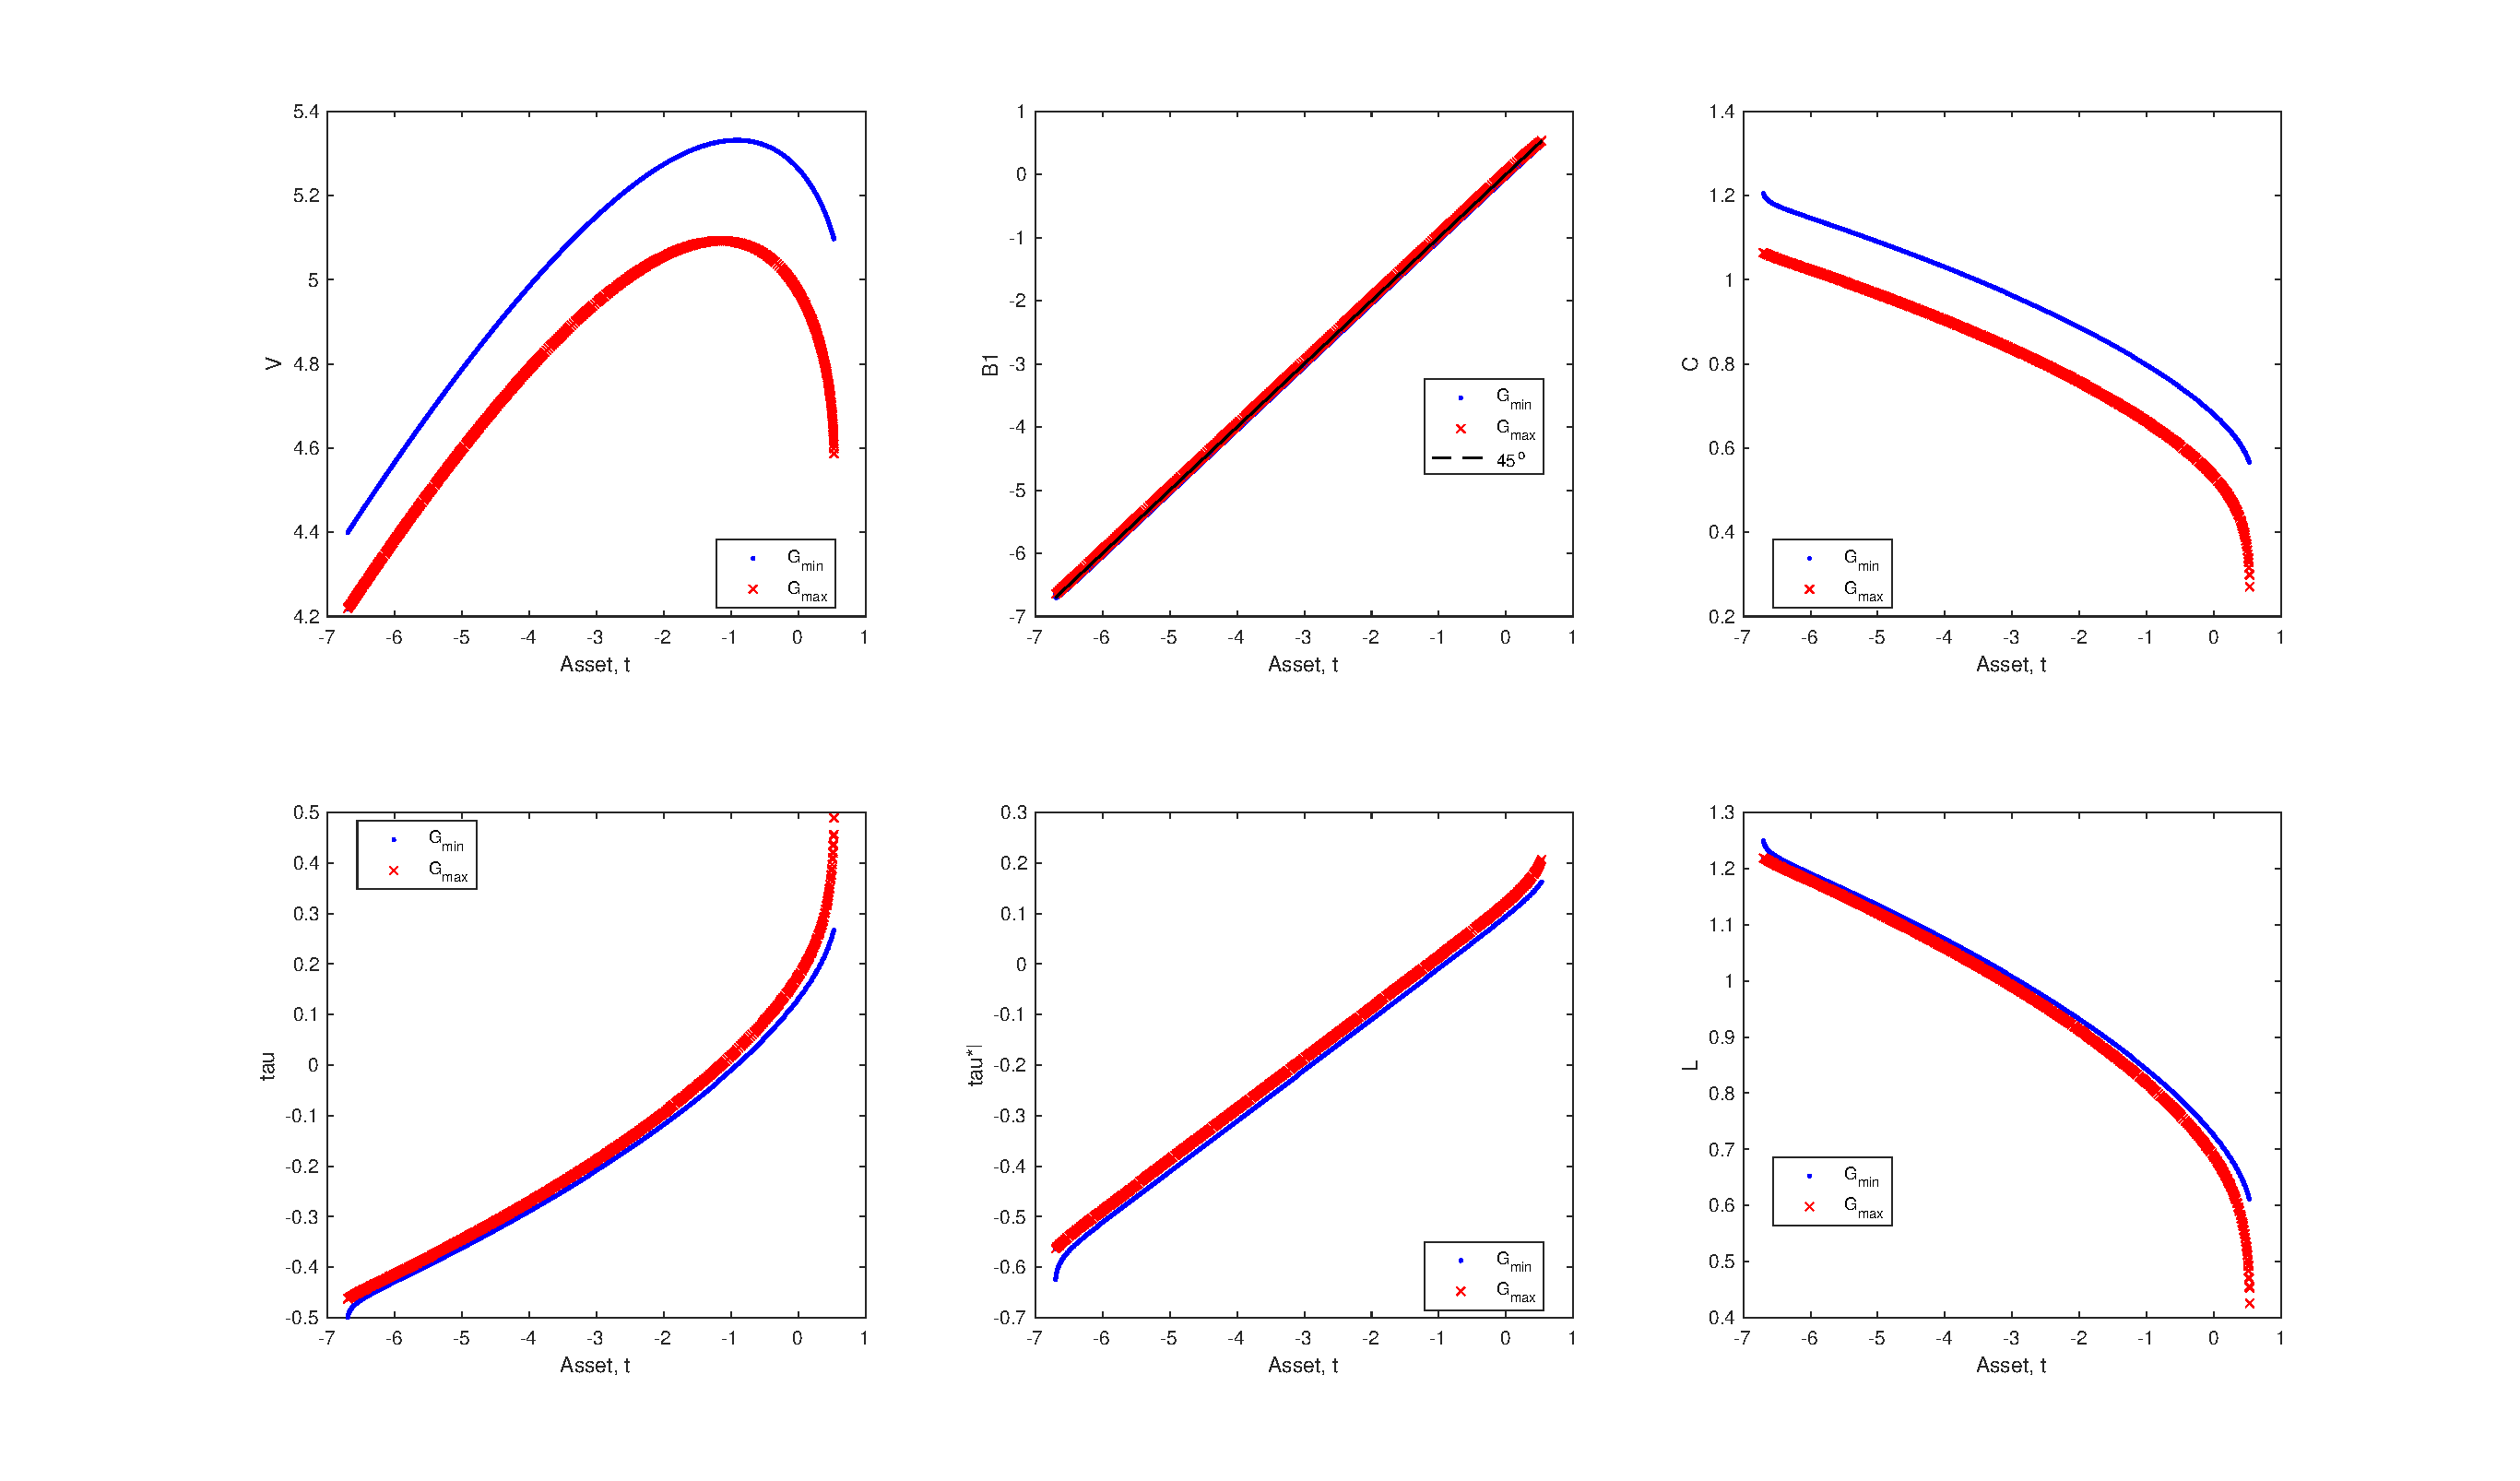
\includegraphics[width=0.92\textwidth]{equm_632}\\
{\scriptsize Equilibrium functions (appendix, $\underline{B}=-6.8$, $\tau\ge-0.5$):
the non-monotonicity of $V$ and the sign reversal of $V_B$ are more pronounced at a
looser asset ceiling. Source: Feng--Han--Zhu.}
\end{center}
\end{column}
\end{columns}
\end{frame}

\begin{frame}{RA Findings II: Ergodic Debt Dynamics Inside Endogenous Limits}
\begin{columns}[T]
\begin{column}{0.50\textwidth}
\small
\textbf{Long-run fiscal behavior in the quasi-linear case:}
\begin{itemize}
    \item Taxes and debt follow \textbf{Barro (1979)-style random-walk dynamics} --- but confined
          to endogenous limits $[\underline{B}, \bar{B}]$
    \item A \textbf{unique ergodic stationary distribution} of debt exists (extends Bhandari
          et al.\ 2017 to Markov spending)
    \item The debt ceiling $\bar{B}$ is approached but never reached; the asset ceiling
          $\underline{B}$ binds with positive probability (mass point)
    \item No convergence to the complete-markets Lucas--Stokey allocation
\end{itemize}

\smallskip
\textbf{Learned jointly with the solution:} the admissible set $\Omega$ --- the ancestor of the
viability kernel in the HA model.
\end{column}
\begin{column}{0.47\textwidth}
\begin{center}
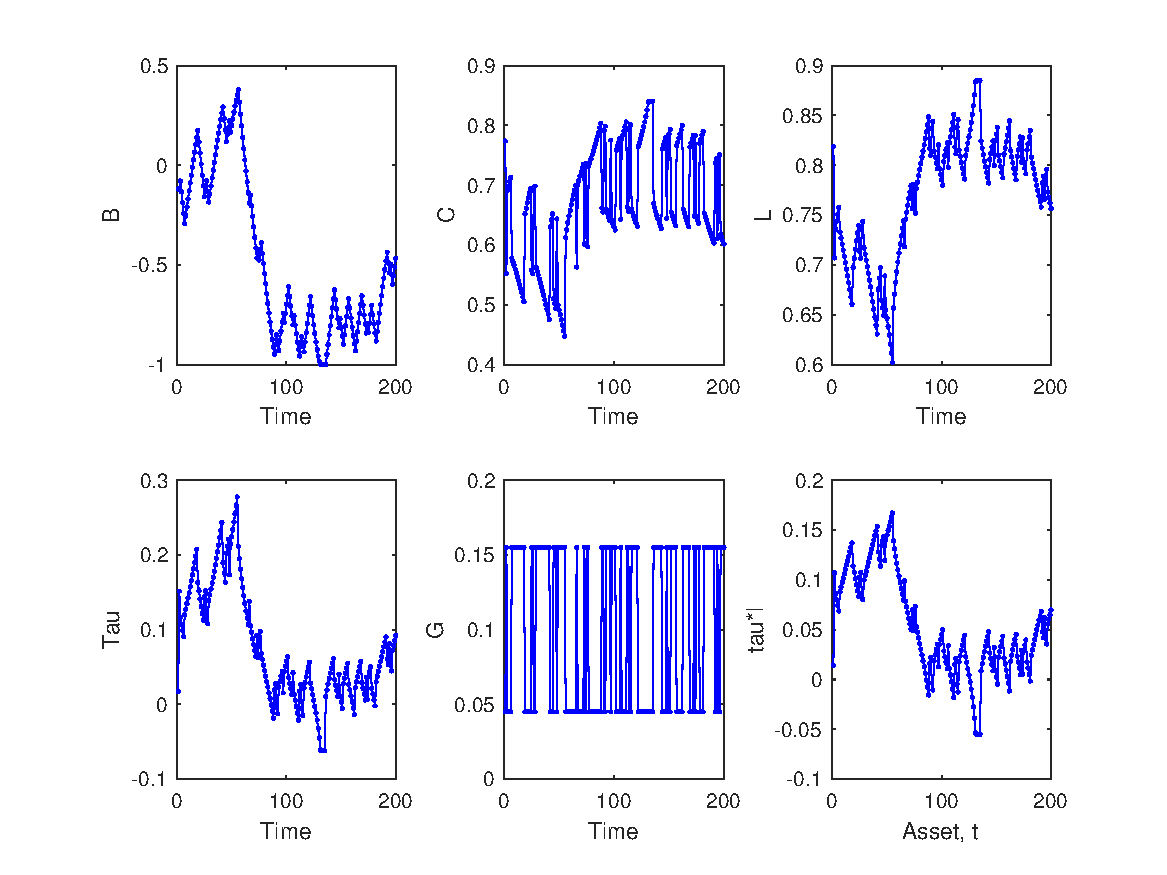
\includegraphics[width=0.92\textwidth]{sim_633}\\
{\scriptsize Simulated paths, baseline economy ($\underline{B}=-1$): persistent fluctuations of
debt and taxes inside the endogenous limits; the lower bound binds intermittently.
Source: Feng--Han--Zhu.}
\end{center}
\end{column}
\end{columns}
\end{frame}

\begin{frame}{HA Findings I: Front-Loaded Transition to Full Self-Insurance (CRRA)}
\begin{columns}[T]
\begin{column}{0.50\textwidth}
\textbf{Section 7, CRRA ($\sigma=\gamma=2$):} the long-run target is \textbf{boundary full
self-insurance (FSI)} --- equal consumption $c^e = c^u = 0.669$, $Q=\beta$, $\tau_n = 0.2$,
unemployed constraint binding.

\medskip
\textbf{The transition is sharply front-loaded:}
\begin{itemize}
    \item the planner \emph{immediately} issues debt to build the bond stock households need
          to self-insure
    \item early borrowing is \textbf{cheap}: at $t=0$ the labor tax is a \emph{subsidy}
          ($\tau_n < 0$) and bond prices are high
    \item two reinforcing forces: Lucas--Stokey interest-rate manipulation $+$ the
          precautionary/liquidity premium ($Q > \beta$); both vanish as FSI is reached
\end{itemize}
\end{column}
\begin{column}{0.47\textwidth}
\begin{center}
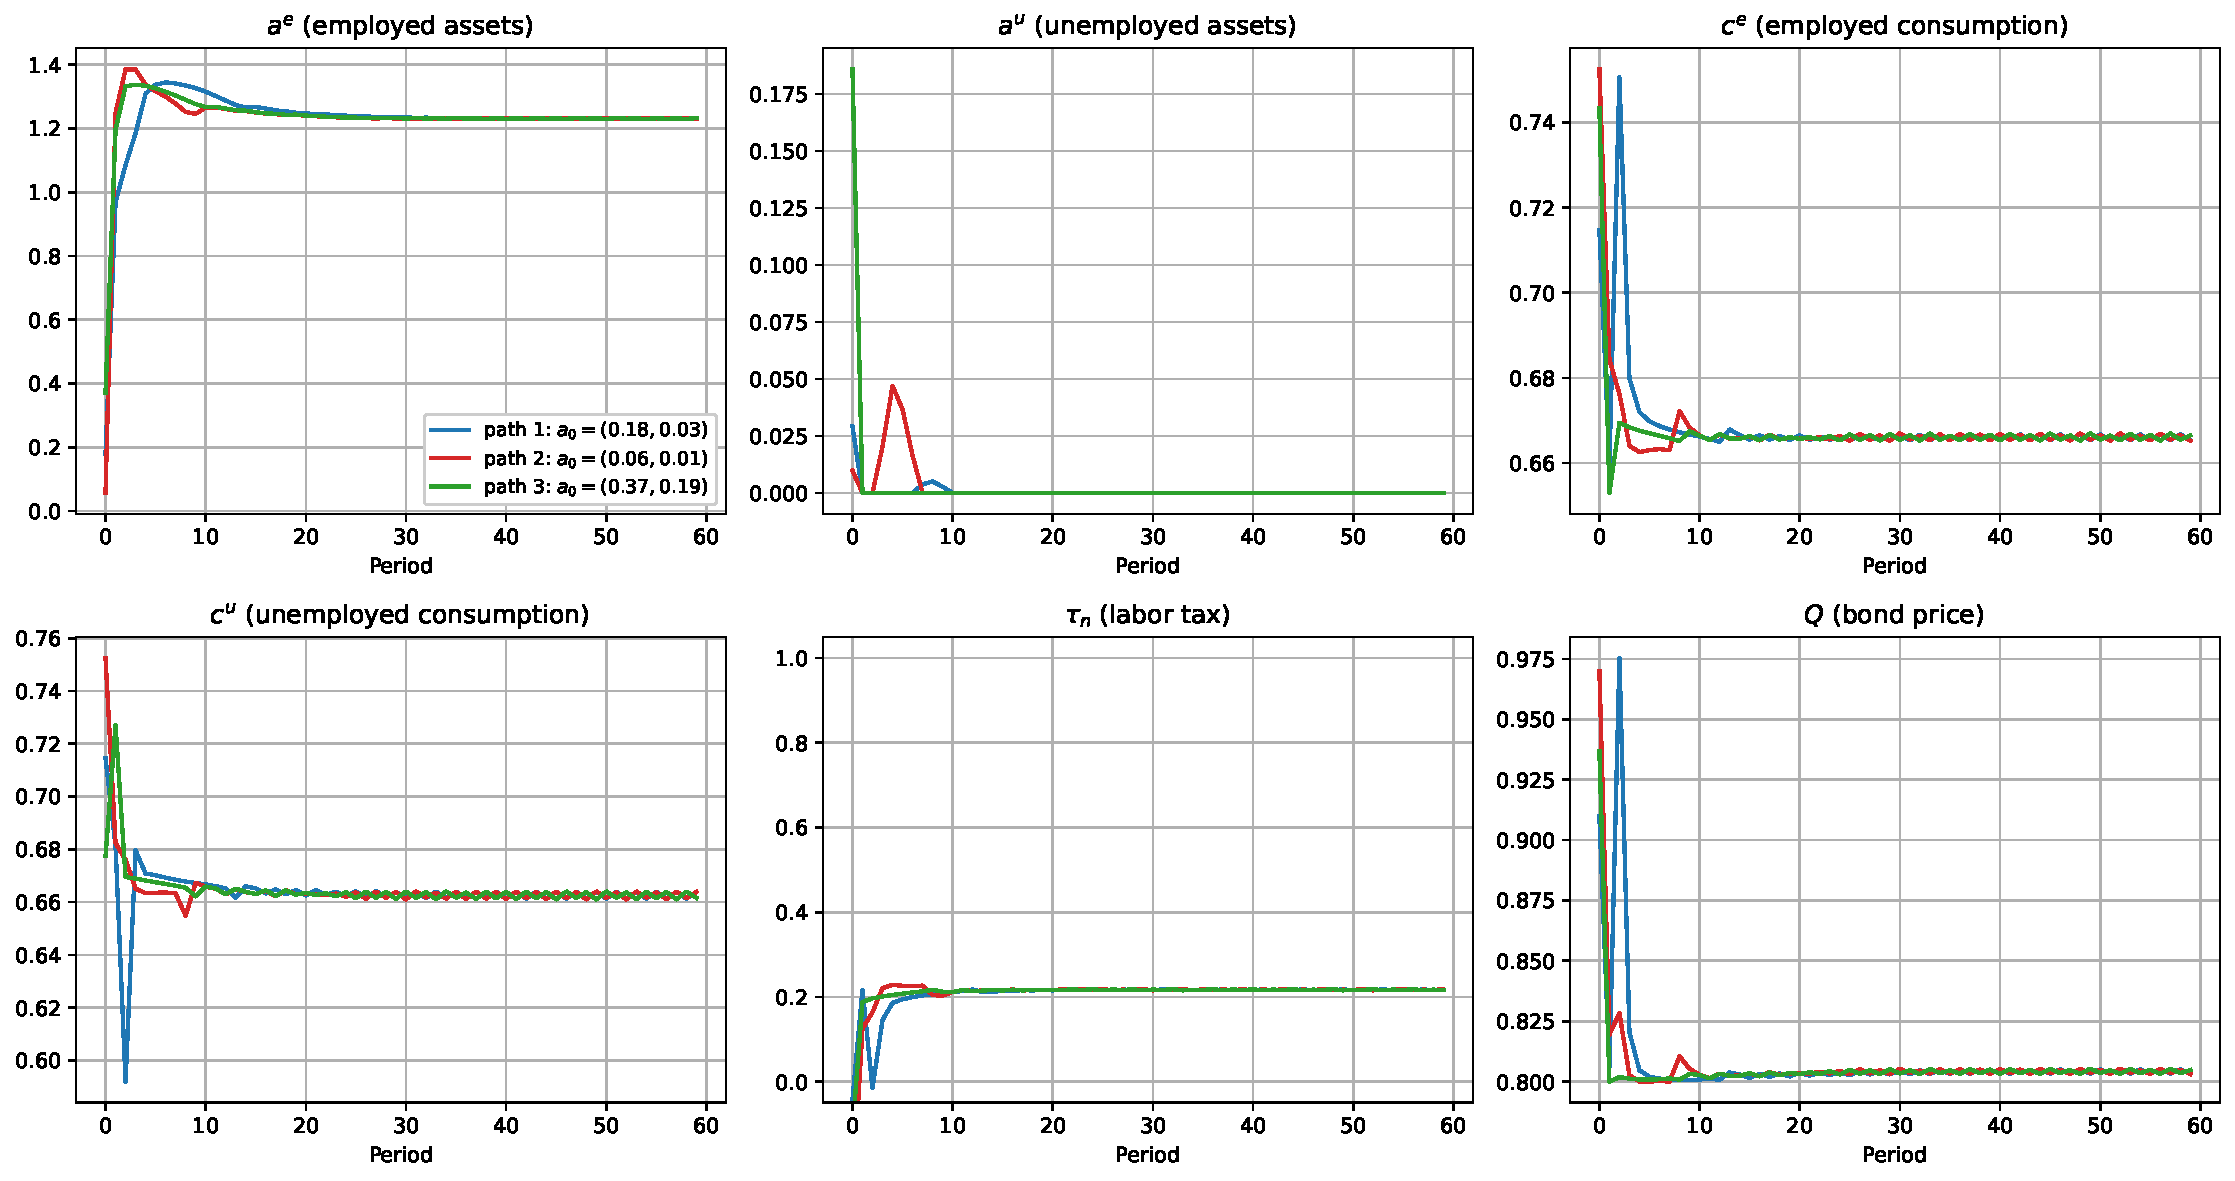
\includegraphics[width=\textwidth]{crra_v6_converge}\\
{\scriptsize CRRA transition: assets, consumptions, labor tax, and bond price over 60 periods ---
debt buildup, initial subsidy, convergence to equal consumption with $Q\to\beta$.
Source: Chien--Feng--Wen, Section 7.}
\end{center}
\end{column}
\end{columns}
\end{frame}

\begin{frame}{HA Findings II: Bistability --- FSI or Immiseration}
\begin{columns}[T]
\begin{column}{0.46\textwidth}
\small
\textbf{The economy has \emph{two} long-run outcomes:} the FSI steady state and
\textbf{immiseration} (assets pile up, consumption collapses, $\tau_n \to 1$).

\smallskip
\begin{itemize}
    \item Which one is reached depends on \textbf{where the economy starts}
    \item CRRA: only $\approx 13\%$ of initial conditions (a \emph{thin low-asset sliver})
          converge to FSI; GHH: $\approx 28\%$
    \item Basin boundaries are thin and perturbation-sensitive --- mapped with the
          $\alpha$-shape machinery from Milestone 5
\end{itemize}

\smallskip
\begin{block}{Long-run outcomes are history-dependent}
Policy alone does not decide between
self-insurance and immiseration --- initial conditions do.
\end{block}
\end{column}
\begin{column}{0.52\textwidth}
\begin{center}
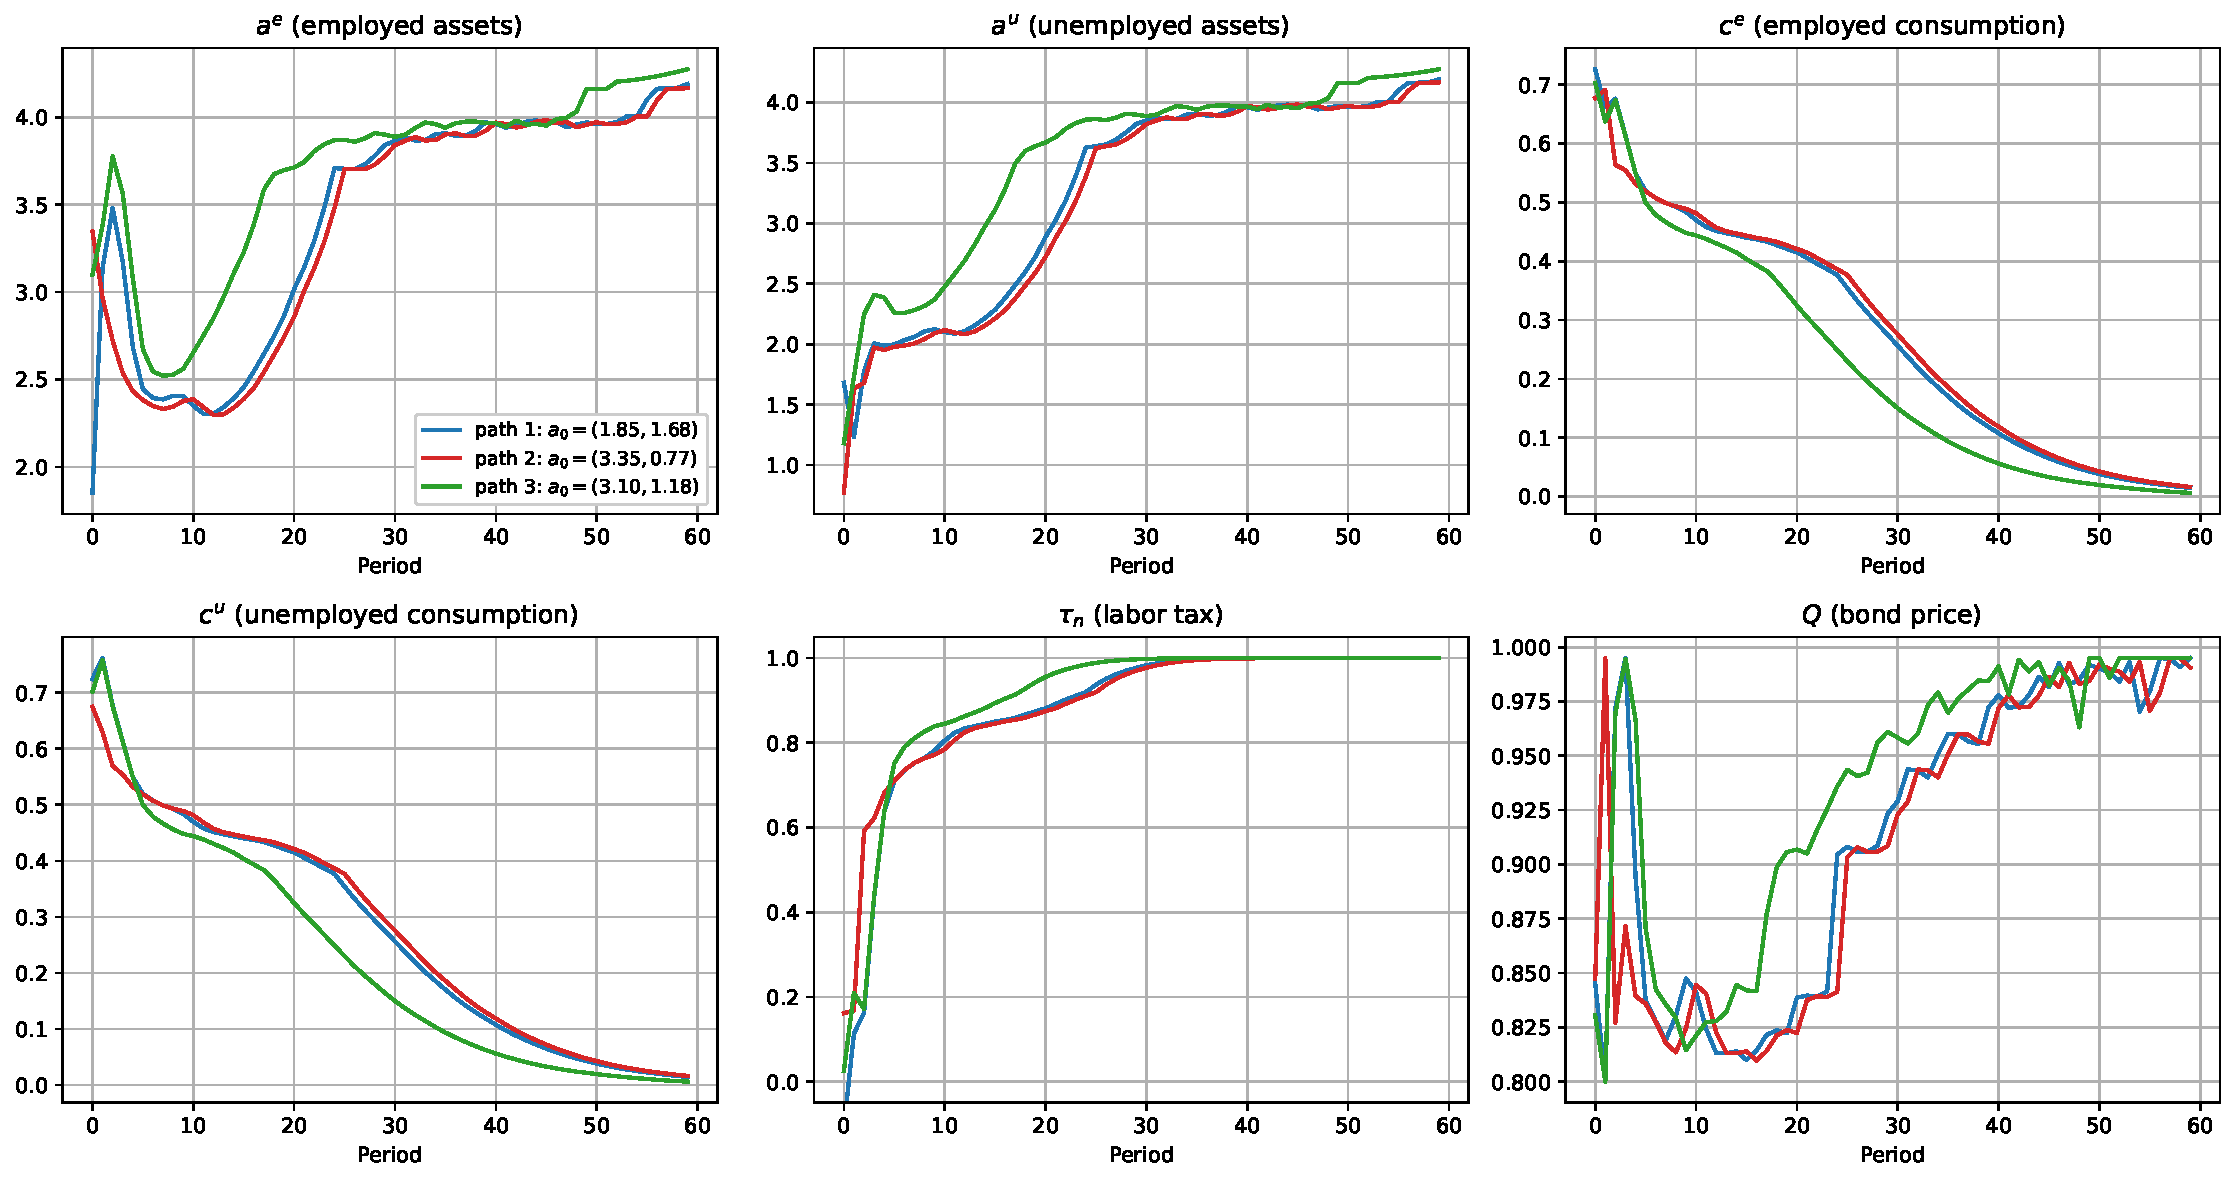
\includegraphics[width=\linewidth]{crra_v6_diverge}\\[0.2em]
{\scriptsize Immiseration path from high initial assets ($a^e_0, a^u_0$ large):
assets accumulate without bound, consumption collapses, $\tau_n\to1$.
Source: Chien--Feng--Wen.}
\end{center}
\end{column}
\end{columns}
\end{frame}

\begin{frame}{What Heterogeneity Adds: RA vs.\ HA Side by Side}
\compacttables
\begin{center}\footnotesize
\renewcommand{\arraystretch}{1.0}
\begin{tabular}{p{3.0cm}p{4.4cm}p{4.7cm}}
\toprule
& \textbf{RA, quasi-linear (seed)} & \textbf{HA, CRRA (new)} \\
\midrule
Role of public debt & smooth tax distortions over time & \emph{also} supply liquid assets for household self-insurance \\
Long-run behavior & ergodic fluctuations inside endogenous debt limits & convergence to full self-insurance --- \emph{or} immiseration \\
History dependence & initial debt selects a stationary \emph{regime} (log case) & initial state selects the \emph{long-run outcome} itself (thin basin) \\
Interest-rate channel & price effects via $q$; negative rates when asset-rich & Lucas--Stokey manipulation of the \emph{risk-free} rate $+$ precautionary premium \\
Redistribution & none (representative agent) & transition engineered to lift the unemployed off the borrowing limit \\
Key constraint object & admissible set $\Omega(z)$ in $(B,\lambda)$ & viability kernel in 4--5D, non-convex, learned by $\alpha$-shapes \\
\bottomrule
\end{tabular}
\end{center}

\smallskip
\begin{block}{}
\small \textbf{The new economics is not ``RA plus noise.''} Heterogeneity changes what debt is \emph{for},
creates a bistable long run, and makes the feasible-set geometry an object of interest.
\end{block}
\end{frame}

% ============================================================
\section{Lessons}
% ============================================================

\begin{frame}{A Paradigm Shift in Economic Research}
\textbf{What changed, concretely, relative to the pre-AI workflow:}

\medskip
\begin{itemize}
    \item \textbf{The theory--code--debug loop compressed} from months to days: drafting,
          refactoring, auditing, and diagnostics summarization are no longer bottlenecks
    \item \textbf{Documentation became executable}: the TeX spec, the audit notes, and the
          code evolve in lockstep because the agent keeps them synchronized
    \item \textbf{Cross-literature imports got cheap}: computational geometry ($\alpha$-shapes),
          viability theory (Aubin), and control-theoretic stability (Lyapunov) entered an
          economics project through iteration, not through years of retooling
    \item \textbf{The unit of progress is the validated milestone}, not the finished paper ---
          and every milestone is preserved, reproducible, and auditable
\end{itemize}

\medskip
\begin{alertblock}{}
What did \emph{not} change: the AI never decided what was economically interesting,
never noticed on its own that an equation had the wrong timing, and never knew when a
numerical result was not credible. Those calls remained human at every milestone.
\end{alertblock}
\end{frame}

\begin{frame}{To Benefit the Most, You Need Four Things}
\begin{enumerate}
    \item \textbf{A good seed.} A model--algorithm--code triple that already works, is documented,
          and has the potential to extend toward the problem you want to solve.
          \emph{(Here: the RA deep Ramsey solver.)}
    \medskip
    \item \textbf{A clear vision.} Know which problem is interesting, why, and how it builds on
          what you have. \emph{(Here: what does optimal debt policy look like when households
          actually need the debt to self-insure?)}
    \medskip
    \item \textbf{Good judgment.} Steer the research: accept or reject formulations, catch
          economically wrong but plausible equations, decide which simplifications are strategic
          and which are fatal. \emph{(Here: the timing bug, the transition-direction bug, the
          decision to strip down before scaling up.)}
    \medskip
    \item \textbf{Orchestration.} Run different AI agents/sessions on different layers ---
          formalization, implementation, auditing, sweeps, write-up --- and integrate their
          outputs toward your goal. \emph{(Here: separate conversations for model drafting,
          code review, debugging, and documentation, all feeding one package.)}
\end{enumerate}
\end{frame}

\begin{frame}{The Workflow Is the Product}
\compacttables
\begin{center}\footnotesize
\renewcommand{\arraystretch}{1.0}
\begin{tabular}{p{5.6cm}p{6.3cm}}
\toprule
\textbf{You provide} & \textbf{AI provides} \\
\midrule
the seed and the destination & speed between them \\
economic correctness & syntactic and structural correctness \\
acceptance criteria at each milestone & candidate artifacts to accept or reject \\
the question ``is this credible?'' & the diagnostics to answer it \\
\bottomrule
\end{tabular}
\end{center}

\smallskip
\begin{block}{}
\small \textbf{The path:} working RA solver $\to$ audit and refine $\to$ stripped-down HA model
$\to$ AI-built prototype $\to$ full research code $\to$ three new discoveries
($\alpha$-shapes, viability kernel, Lyapunov design) $\to$ new economics
(debt as liquidity, bistable long run, history dependence).
\end{block}

\smallskip
{\small\textbf{Everything is replicable from \texttt{Case\_Study/}:} the code at every
milestone, the TeX at every version, the audits, and the conversation provenance.}

\smallskip
\scriptsize\textit{References: Feng--Han--Zhu (Ramsey taxation \& debt sustainability);
Chien--Feng--Wen (HA Ramsey, Sec.~7); Chien--Feng (computational methods note);
AMSS (2002); Barro (1979); Lucas--Stokey (1983); Abreu--Pearce--Stacchetti (1990);
Aubin (1991); Saint-Pierre (1994); Edelsbrunner--M\"ucke (1994); Phelan--Stacchetti (2001); Feng (2015).}
\end{frame}

% ============================================================
\begin{frame}[standout]
  Thank you.\\[6mm]
  Questions?
\end{frame}

% ============================================================
\appendix
% ============================================================

% -------- A1: RA Recursive Planner Problem ------------------
\begin{frame}[label=appRAprob]{Appendix A1 --- RA: Recursive Planner Problem}
\hfill\hyperlink{mainRAalgo}{\beamerreturnbutton{Return}}
\vspace{0.2em}

\textbf{State} $S=(z,B,\lambda)$: spending shock, govt.\ bonds/assets, promised marginal utility.
\textbf{Control}: contingent next-period co-states $\{\lambda_+(z_+)\}$.

\smallskip
\textbf{Continuation Bellman (P-1), $t\ge1$:}
\vspace{-0.2cm}
\[
V(z,B,\lambda)=\max_{\{\lambda_+(z_+)\}}\Big\{u(c)-h(l)+\beta\,\mathbb{E}\big[V(z_+,B_+,\lambda_+)\big]\Big\}
\]
\vspace{-0.4cm}
\begin{align*}
G(z)+B &\le \tau l + qB_+, \quad c+G(z)=l, \quad u'(c)=\lambda \\
(1-\tau)u'(c)&=h'(l), \quad qu'(c)=\beta\,\mathbb{E}[\lambda_+\mid z]\\
(B,\lambda)&\in\Omega(z), \quad (B_+,\lambda_+)\in\Omega(z_+)
\end{align*}

\textbf{Period-0 problem (P-2)}: identical but $\lambda$ is not an inherited state --- the promise-keeping
constraint $u'(c)=\lambda$ is absent; the planner sets initial distortions freely.

\smallskip
\begin{block}{Admissible set $\Omega(z)$}
\small The set of $(B,\lambda)$ pairs from which the government can remain solvent indefinitely.
\emph{Unknown a priori} --- determined jointly with the policy as a fixed point of the
classification procedure. Quasi-linear case: $\lambda\equiv1$, $q=\beta$; state collapses to $(z,B)$.
\end{block}
\end{frame}

% -------- A2: RA Algorithm Details --------------------------
\begin{frame}[label=appRAalgo]{Appendix A2 --- RA: DNN Two-Level Fixed-Point Algorithm}
\hfill\hyperlink{mainRAalgo}{\beamerreturnbutton{Return}}
\vspace{0.2em}

\textbf{Three DNNs:} $f_\Lambda$ (policy), $f_V$ (value), $f_\Omega$ (admissible-set classifier).
\textbf{Outer iteration $n$:}

\smallskip
\compacttables\footnotesize
\begin{tabular}{p{0.9cm}p{10.9cm}}
\toprule
\textbf{Step 1} & \textbf{Policy + value update.} Given $\Omega^{(n)}$: rejection-sample $N_1$ states $S_{i,0}$ from
$\mathcal{H}$ (accept if $f_\Omega(S_{i,0})\ge\varsigma_i\sim\mathcal{U}[0,1]$). Simulate $T_V$-period rollouts
$\Rightarrow$ realized utilities $\hat V(S_{i,0})=\sum_{t=0}^{T_V-1}\beta^t[u(c_{i,t})-h(l_{i,t})]$.
Fit $f_V^{(n+1)}$ via MSE. Update $f_\Lambda^{(n+1)}$ by maximizing
$\mathbb{E}\big[\sum_t\beta^t(u(c_t)-h(l_t)-\kappa[1-f_\Omega(S_t)])+\beta^{T_\Lambda}f_V(S_{T_\Lambda})\big]$
via SGD. \\[0.3em]
\textbf{Step 2} & \textbf{Admissible-set update.} Simulate from updated policy; for each state $S_{i,t}$
label $\chi^{\Omega,(n+1)}(S_{i,t})=1$ iff (i) $S_{i,t+1}\in\Omega^{(n)}$ and (ii) $V(S_{i,t})$ finite.
Fit $f_\Omega^{(n+1)}$ to this binary dataset via MSE. \\
\bottomrule
\end{tabular}

\smallskip
Repeat until $f_\Lambda$, $f_V$, $f_\Omega$ all converge. The key innovation vs.\ grid methods:
$f_\Omega$ learns the \emph{characteristic function} of $\Omega$ --- no convexity, no grid, scales to higher dimensions.
\end{frame}

% -------- B1: HA Model Equilibrium Conditions ---------------
\begin{frame}[label=appHAmodel]{Appendix B1 --- HA Model: Analytical Forward Map}
\hfill\hyperlink{mainM2}{\beamerreturnbutton{Return}}
\vspace{0.2em}

\textbf{Two states} $i\in\{e,u\}$; stationary weights $(\pi^e,\pi^u)$; Markov transitions $\Pi=(\pi^{ij})$.
Linear technology ($K\equiv1$, $\alpha=\delta=0$); state $s=(a^e,a^u,c^e,c^u)$; controls $(c'^e,c'^u)$.
\textbf{All other equilibrium objects follow analytically:}
\begin{align*}
n^e &= c^e + \tfrac{\pi^u}{\pi^e}c^u & &\text{(labor market clearing)}\\
\hat w &= (n^e)^\gamma(c^e)^\sigma & &\text{(after-tax wage)}\\
Q &= \beta(c^e)^\sigma\!\left(\tfrac{\pi^{ee}}{(c'^e)^\sigma}+\tfrac{\pi^{eu}}{(c'^u)^\sigma}\right) & &\text{(bond price)}\\
a'^e &= \tfrac{1}{Q}\!\left[\tfrac{a^e\pi^e\pi^{ee}+a^u\pi^u\pi^{ue}}{\pi^e}+\hat w\,n^e-c^e\right] & &\text{(employed asset transition)}\\
a'^u &= \tfrac{1}{Q}\!\left[\tfrac{a^e\pi^e\pi^{eu}+a^u\pi^u\pi^{uu}}{\pi^u}-c^u\right] & &\text{(unemployed asset transition)}
\end{align*}

\textbf{Borrowing constraints + KKT:} Define Euler discrepancy
$\tilde\phi^i\equiv Q/(c^i)^\sigma - \beta\sum_j\pi^{ij}/(c'^j)^\sigma$. Then:
\begin{equation} \label{eq:kkt}
a'^i\ge0,\quad \tilde\phi^i\ge0,\quad a'^i\tilde\phi^i=0,\qquad i\in\{e,u\}.
\end{equation}
\end{frame}

% -------- B2: HA Recursive Problem + Viability Challenge ----
\begin{frame}[label=appHArec]{Appendix B2 --- HA: Recursive Problem and Viability Challenge}
\hfill\hyperlink{mainM2fb}{\beamerreturnbutton{Return}}
\vspace{0.2em}

\textbf{Continuation Bellman ($t\ge1$):} state $s_t=(a^e_t,a^u_t,c^e_t,c^u_t)$, controls $(c'^e,c'^u)$:
\[
V(s_t)=\max_{c'^e,c'^u}\Big\{\pi^e u(c^e_t,n^e_t)+\pi^u u(c^u_t,0)+\beta\,V(s_{t+1})\Big\}
\]
subject to the analytical forward map $s_{t+1}=f(s_t,y_t)$, feasibility, and KKT \eqref{eq:kkt}.
The period-0 problem differs: no inherited promises, so $(c^e_0,c^u_0)$ are chosen freely.

\smallskip
\textbf{The viability challenge.} The admissible domain is the \emph{viability kernel}:
\[
\Omega = \big\{s\in H:\exists\,y\ \text{s.t.}\ f(s,y)\in\Omega\ \text{and borrowing/KKT hold}\big\}.
\]
It is the \textbf{largest fixed point} of the feasibility operator
$\mathcal{T}(D)=\{s\in D:\exists\,y\ \text{s.t.}\ f(s,y)\in D,\ \text{constraints hold}\}$,
computed by inward iteration $D^{k+1}=\mathcal{T}(D^k)\downarrow\Omega^*$ from $D^0=H$.

\begin{alertblock}{The central computational challenge}
\small $\Omega$ depends on the policy, which depends on $\Omega$ --- the planner's problem is
well-defined only on $\Omega$. This circularity requires the domain to be learned jointly with
the policy: the fixed-point structure of the RA DNN approach carries over, but the
\emph{representation} of $\Omega$ must change (from a 2D admissibility function to a 4--5D geometry).
\end{alertblock}
\end{frame}

% -------- C1: Fischer-Burmeister Complementarity ------------
\begin{frame}[label=appFB]{Appendix C1 --- Algorithm: Fischer--Burmeister Complementarity}
\hfill\hyperlink{mainFinalAlgo}{\beamerreturnbutton{Return}}
\vspace{0.2em}

\textbf{Problem:} gradient-based optimizers cannot enforce hard complementarity $a'^i\ge0$,
$\tilde\phi^i\ge0$, $a'^i\tilde\phi^i=0$ directly. We use a differentiable surrogate.

\smallskip
\textbf{Consumption-scaled Euler discrepancy} (preserves sign, stabilizes magnitudes):
$\phi^i=(c^i)^\sigma\tilde\phi^i$.

\smallskip
\textbf{Smoothed Fischer--Burmeister function:}
\[
\Phi_\varepsilon(\mu,a)=\mu+a-\sqrt{\mu^2+a^2+\varepsilon^2},\quad\varepsilon>0.
\]
$\Phi_\varepsilon\to0$ iff $\mu\ge0$, $a\ge0$, $\mu a=0$ as $\varepsilon\downarrow0$. Feed it the
\emph{rectified} discrepancy $\mu=[\phi^i]_+$ and asset $a=a'^i$.

\smallskip
\textbf{Rectification is not enough.} It makes the FB residual blind to Euler-sign violations
($\phi^i<0$). Two supplementary penalties:
\[
\mathcal{P}_{ineq}=\mathbb{E}\textstyle\sum_{t,i}[-\phi^i_t]_+^2\quad\text{(Euler inequality guard)},
\qquad
\mathcal{P}_{int}=\mathbb{E}\textstyle\sum_{t,i}(1-b^i_t)(\phi^i_t)^2\quad\text{(interior equality)},
\]
where $b^i_t=\mathbf{1}\{a'^{i,\text{raw}}\le\bar a\}$ is the binding indicator.

\smallskip
\textbf{Stabilized primitives} prevent numerical explosions during training:
sigmoid clamp on $c'^i$ (keeps consumption in $[c_{\min},c_{\max}]$);
$Q$-clipping; softplus enforcement of $a'^i\ge0$.
\end{frame}

% -------- C2: Domain Learning --------------------------------
\begin{frame}[label=appDomain]{Appendix C2 --- Algorithm: Domain Learning via $\alpha$-Shapes}
\hfill\hyperlink{mainFinalAlgo}{\beamerreturnbutton{Return}}
\vspace{0.2em}

\textbf{Admissibility score.} For each candidate $s$ sampled from the hypercube $H$:
\[
\mathcal{A}(s;\theta,\Omega)=w_{geo}\,\mathbf{1}\!\big\{f_\theta(s)\in\Omega\big\}
+w_Q\,\mathcal{B}(Q^{raw}(s))
\]
where the first term is a geometric feasibility check (does the policy-implied successor lie
inside $\Omega$?) and $\mathcal{B}$ penalizes economically implausible raw bond prices.
States with $\mathcal{A}>\tau_A$ form the training pool $\mathcal{D}_{train}$.

\smallskip
\textbf{$\alpha$-shape boundary reconstruction} (Edelsbrunner--M\"ucke 1994):
\[
\Omega\leftarrow\mathrm{AlphaShape}(\mathcal{D}_{train};\,\alpha)
\]
the union of Delaunay simplices with circumradius $\le1/\alpha$.
No convexity required --- the viability kernel is generically non-convex (borrowing kink).
$\alpha$ tunes resolution: $\alpha\to0$ gives the convex hull; large $\alpha$ traces concavities.

\smallskip
\textbf{Projection $\Pi_\Omega$.} Out-of-domain rollout successors are projected back to the
nearest admissible point. A \emph{projection-distance penalty} prevents the actor from relying on
this silent correction. Boundary + training pool are refreshed every $\sim$20 iterations
(amortized to control non-stationarity).
\end{frame}

% -------- C3: Lyapunov Penalty --------------------------------
\begin{frame}[label=appLyap]{Appendix C3 --- Algorithm: Lyapunov Penalty for Saddle-Path Selection}
\hfill\hyperlink{mainFinalAlgo}{\beamerreturnbutton{Return}}
\vspace{0.2em}

\textbf{The problem.} Under the linear-technology calibration $\beta R=1$: the FSI steady state
is \emph{knife-edge neutrally stable}. The total asset level is a unit root.
Euler/FB residuals can be near zero while the simulation drifts --- both the stable manifold
\emph{and} the unstable arm satisfy the first-order conditions pointwise.
A finite-horizon rollout with a bootstrap terminal value cannot distinguish them.

\smallskip
\textbf{What a Lyapunov certificate must look like here:}
\begin{itemize}
  \item Flat along the $c^e=c^u$ ridge (full-insurance manifold) and flat in total-asset level
  \item Positive only \emph{off} the manifold --- penalizing the level itself would wrongly reject
        optimal unit-root dynamics
\end{itemize}

\textbf{The penalty} (run on a closed loop seeded at $s_{FSI}$):
\[
\mathcal{P}_{lyap}=\sum_t\beta^t\Big[\underbrace{w_{spread}(c^e_t-c^u_t)^2}_{\text{manifold-distance certificate}}
+\underbrace{[a^{tot}_t-a^{tot}_{t-1}]_+^2}_{\text{one-sided anti-explosion guard}}\Big],
\quad a^{tot}=\pi^e a^e+\pi^u a^u.
\]

The one-sided guard penalizes explosive asset growth ($>1$ eigenvalue) while remaining
flat for unit-root persistence and pinning no level.
\end{frame}

% -------- C4: Unified Actor Objective (Full Stack) -----------
\begin{frame}[label=appStack]{Appendix C4 --- Algorithm: Unified Actor Objective}
\hfill\hyperlink{mainFinalAlgo}{\beamerreturnbutton{Return}}
\vspace{0.2em}

The actor minimizes $\mathcal{L}_{actor}=\mathbb{E}\big[\sum_{t=0}^{T-1}\beta^t\ell_t-\beta^T V_\psi(s_T)\big]$
with \textbf{stage loss} combining welfare and all complementarity/stability penalties:

\smallskip
\compacttables\footnotesize
\renewcommand{\arraystretch}{1.1}
\begin{tabular}{p{2.5cm}p{4.8cm}p{4.5cm}}
\toprule
\textbf{Term} & \textbf{What it enforces} & \textbf{When it fires} \\
\midrule
$-U(s_t)$ & welfare (maximized) & always \\
$\lambda_{FB}\,|\Phi^i_t|^p$ & FB complementarity residual & always (both types) \\
$\lambda_{bound}\,p_{bound,t}$ & raw-asset excursions above ceiling & near-boundary states \\
$\lambda_{shape}\,d_t^2$ & projection distance (stay in $\Omega$) & out-of-domain rollouts \\
$\lambda_{comp}\sum_i[\phi^i_t]_+[a'^i_t]_+$ & ``both positive'' forbidden quadrant & near-kink states \\
$\lambda_{ineq}\sum_i[-\phi^i_t]_+^2$ & Euler-sign guard & Euler violations \\
$\lambda_{int}\sum_i(1-b^i_t)(\phi^i_t)^2$ & interior Euler equality & unconstrained states \\
$\lambda_Q\,p_{Q,t}$ & raw bond-price feasibility & implausible $Q$ \\
$\lambda_{eum}\,b^u_t[\phi^u_{tgt}-\phi^u_t]_+^2$ & unemployed Euler margin & near-binding regime \\
$\lambda_{lyap}\,\mathcal{P}_{lyap}$ & saddle-path selection & full rollout \\
\bottomrule
\end{tabular}

\smallskip
{\small Each penalty term answers a specific failure mode encountered during development.
Penalty weights $\boldsymbol\lambda$ are \emph{fixed multipliers} (augmented Lagrangian style);
$\beta^t$ discounting keeps every term on the same scale as welfare.}
\end{frame}

\end{document}
